\chapter{Kompression}\label{ch:Lektion}
\section{Einführung}

\subsection{Was ist Kompression?}

Der Begriff \enquote{Kompression} stammt --- wie viele andere Begriffe --- ursprünglich aus dem Lateinischen (\textit{compressio} $=$ das Zusammendrücken, die Zusammenpressung, die Umarmung). Mit Kompression ist also häufig die \enquote{Verkleinerung} bzw. das \enquote{Zusammendrücken} von Daten gemeint, meist aus einem der folgenden Gründe:

\begin{enumerate}
	\item \textbf{Speicherplatz sparen}: Speichermedien wie Festplatten verursachen Kosten. Mit Kompression kann der Speicherbedarf minimiert werden --- ähnlich wie beim Packen eines Reisekoffers (siehe \cref{fig:speicherplatz-opt}).
		  \begin{figure}[H]
			  \centering
			  \raisebox{-0.5\height}{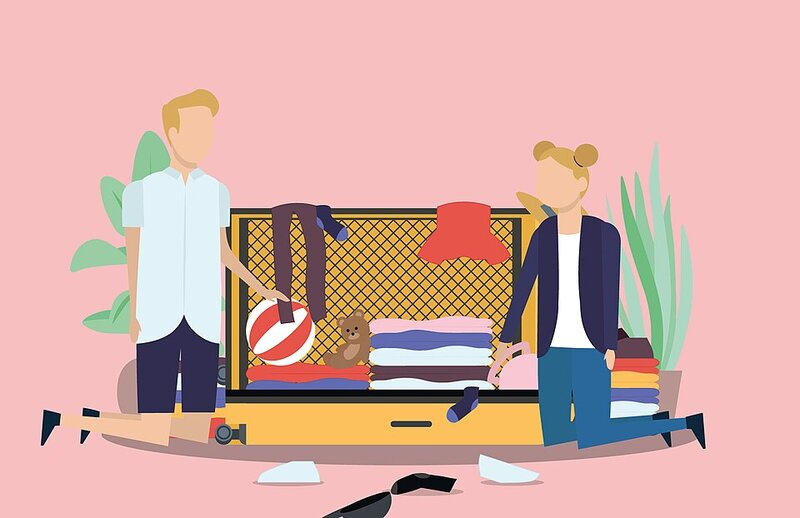
\includegraphics[width=.45\textwidth]{Grundlagen_Info/04_Kompression/Figures/suitcase_messy.jpg}}
			  \raisebox{-0.5\height}{$\rightarrow$}
			  \raisebox{-0.5\height}{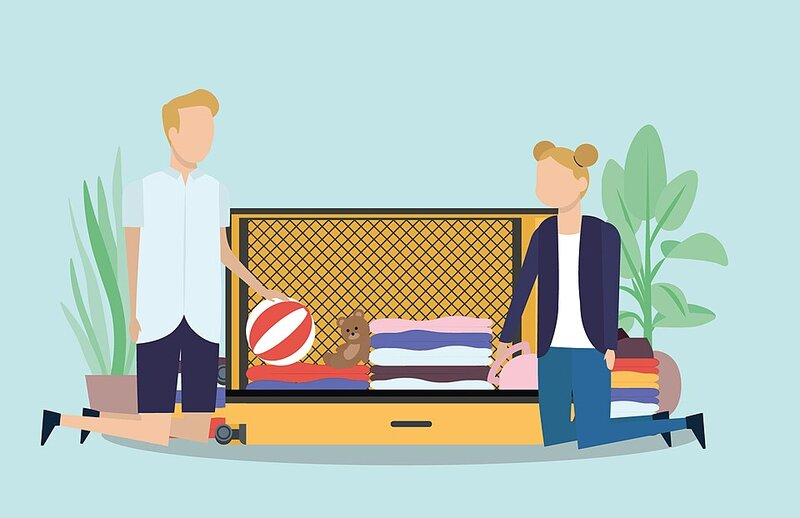
\includegraphics[width=.45\textwidth]{Grundlagen_Info/04_Kompression/Figures/suitcase_packed.jpg}}
			  % Bildquellen: Wikimedia Commons, CC BY 2.0 (Autor im Caption)
			  \caption[Speicherplatz optimieren]{Speicherplatz optimieren. \href{https://commons.wikimedia.org/wiki/File:Messy_Suitcase_Packing_for_a_Holiday.jpg}{\color{RoyalBlue}\scriptsize[Quelle: Familydestinationsguide.com Images, CC BY 2.0]}, \href{https://commons.wikimedia.org/wiki/File:A_Neatly_Packed_Suitcase_for_a_Holiday.jpg}{\color{RoyalBlue}\scriptsize[Quelle: Familydestinationsguide.com Images, CC BY 2.0]}}
			  \label{fig:speicherplatz-opt}
		  \end{figure}
	\item \textbf{Wartezeit verkürzen}: Computer kommunizieren in Netzwerken, in denen oftmals grosse Datenmengen übertragen werden müssen. Die Verbindungen zwischen den Geräten haben jedoch nur eine begrenzte Kapazität und werden daher häufig als \tib{Flaschenhälse} bezeichnet.
		  \begin{figure}[H]
			  \centering
			  \resizebox{!}{.5\height}{%
				  \begin{tikzpicture}
					  \path[mindmap,concept color=black,text=white]
					  node[concept] {Computer}
					  [clockwise from=0]
					  child[concept color=green!50!black] {
							  node[concept] {Computer}
								  [clockwise from=90]
							  child { node[concept] {Computer} }
							  child { node[concept] {Computer} }
							  child { node[concept] {Computer} }
							  child { node[concept] {Computer} }
						  }
					  child[concept color=blue] {
							  node[concept] {Computer}
								  [clockwise from=-30]
							  child { node[concept] {Computer} }
							  child { node[concept] {Computer} }
						  }
					  child[concept color=red] { node[concept] {Computer} }
					  child[concept color=orange] { node[concept] {Computer} };
				  \end{tikzpicture}}
			  \caption{Visualisierung von Computernetzwerken und deren \textit{Flaschenhälsen}}
		  \end{figure}
\end{enumerate}

\subsection{Historischer Kontext}
Kompression war schon lange vor dem Computer ein Thema. Wer früher etwas festhalten wollte, schrieb auf Pergament aus Tierhaut oder meisselte die Buchstaben in Stein. Beides war teuer und aufwendig. Deshalb kürzte man häufige Wörter ab, auf römischen Inschriften etwa SPQR für \textit{Senatus Populusque Romanus} (Senat und Volk von Rom).

Auch die römischen Zahlen lassen sich kürzer oder länger schreiben. Mit den Zeichen C (100), X (10) und I (1) allein braucht die Zahl \textbf{999} 27 Zeichen:
\begin{center}
	\texttt{CCCCCCCCCXXXXXXXXXIIIIIIIII}\\
	$\downarrow$ mit den Zeichen D (500), L (50) und V (5)\\
	\texttt{DCCCCLXXXXVIIII} (15 Zeichen)\\
	$\downarrow$ mit der Subtraktionsschreibweise: IX $=$ 9, XC $=$ 90, CM $=$ 900\\
	\texttt{CMXCIX} (6 Zeichen)
\end{center}
Die noch kürzere Form \texttt{IM} findet man gelegentlich, sie ist nach den heute üblichen Regeln aber nicht gültig: I darf nur vor V und X stehen, X nur vor L und C und C nur vor D und M.

\section{Verlustfreie vs. verlustbehaftete Kompression}
Bei \tib{verlustfreier} Kompression lässt sich die Originaldatei Bit für Bit wiederherstellen. Bei \tib{verlustbehafteter} Kompression lässt man Informationen weg, die man kaum sieht oder hört. Die Datei wird dadurch deutlich kleiner, das Original lässt sich aber nicht mehr zurückgewinnen. Texte, Programme und Tabellen dürfen nur verlustfrei komprimiert werden, weil schon ein falsches Zeichen den Inhalt verändert. Bei Fotos, Musik und Videos ist ein kleiner Qualitätsverlust meist akzeptabel.

\Cref{table:dateiformate} zeigt einige Beispiele.
\begin{table}[H]
	\centering
	\small
	\begin{tabular}{llll}
		\textbf{Anwendung}  & \textbf{Unkomprimiert}             & \textbf{Verlustfrei}                          & \textbf{Verlustbehaftet}                    \\\midrule
		\textbf{Audio}      & \texttt{.wav} (meist)              & \texttt{.flac}                                & \texttt{.mp3}, \texttt{.aac}                \\
		\textbf{Dateien}    & --                                 & \texttt{.zip}, \texttt{.rar}                  & --                                          \\
		\textbf{Video}      & --                                 & selten                                        & \texttt{.mp4}, \texttt{.mov}, \texttt{.avi} \\
		\textbf{Fotografie} & \texttt{.bmp}, \texttt{.raw} (meist) & \texttt{.png}, \texttt{.psd}, \texttt{.webp} & \texttt{.jpg}, \texttt{.webp}               \\
		\textbf{Grafik}     & --                                 & \texttt{.svg}, \texttt{.pdf} (Vektorgrafik)   & --
	\end{tabular}
	\caption{Dateiformate und ihre Kompression}
	\label{table:dateiformate}
\end{table}
Einige Formate lassen sich nicht eindeutig einordnen. \texttt{.wav}-Dateien enthalten meist unkomprimierte Audiodaten, \texttt{.raw}-Dateien die Rohdaten des Bildsensors einer Kamera, je nach Hersteller unkomprimiert oder komprimiert. \texttt{.webp} gibt es verlustfrei und verlustbehaftet. \texttt{.mp4}, \texttt{.mov} und \texttt{.avi} sind \tib{Container}: Sie legen fest, wie Bild, Ton und Untertitel in einer Datei abgelegt sind. Komprimiert wird das Video darin von einem \tib{Codec} (z.\,B. H.264), meistens verlustbehaftet.

\Cref{fig:logo-jpeg-pdf} zeigt das FreeFlower-Logo zweimal. Links wurde es als JPEG mit starker Kompression gespeichert. In der Vergrösserung sieht man an den Kanten der Schrift Kästchen und Farbsäume, sogenannte \tib{Kompressionsartefakte}. JPEG lässt feine Details weg, was bei Fotos kaum auffällt, an scharfen Kanten aber schon. Rechts ist dasselbe Logo als \gls{PDF} gespeichert. Die \acrshort{PDF}-Datei beschreibt die Formen als Vektorgrafik (Linien, Kreise, Buchstaben) und bleibt bei jeder Vergrösserung scharf. Sie ist mit 9 KB auch kleiner als die JPEG-Datei mit 21 KB.

\begin{figure}[H]
	\centering
	\begin{subfigure}{.45\linewidth}
		\centering
		\begin{tikzpicture}
			\node[anchor=south west, inner sep=0] (img) {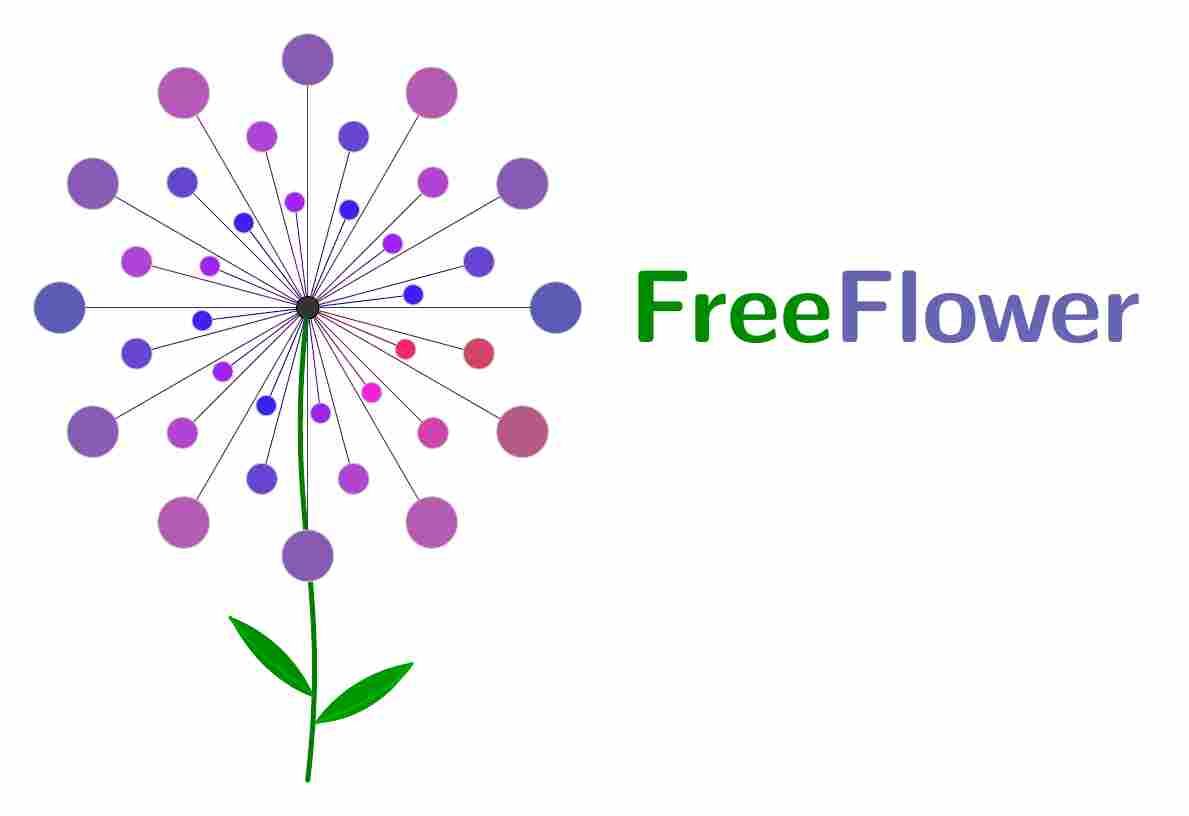
\includegraphics[width=\linewidth]{Grundlagen_Info/04_Kompression/Figures/FreeFlowerLogo.jpg}};
			% roter Rahmen = Ausschnitt der Vergrösserung (relative Koordinaten im Bild)
			\begin{scope}[x=(img.south east), y=(img.north west)]
				\draw[red, thick] (0.538,0.602) rectangle (0.606,0.675);
			\end{scope}
		\end{tikzpicture}
		\caption{JPEG, 21 KB}
	\end{subfigure}\hfill
	\begin{subfigure}{.45\linewidth}
		\centering
		\begin{tikzpicture}
			\node[anchor=south west, inner sep=0] (img) {\includegraphics[width=\linewidth]{Logos/FreeFlower.pdf}};
			\begin{scope}[x=(img.south east), y=(img.north west)]
				\draw[red, thick] (0.538,0.602) rectangle (0.606,0.675);
			\end{scope}
		\end{tikzpicture}
		\caption{\glsentryshort{PDF}, 9 KB}
	\end{subfigure}\\[\baselineskip]
	\begin{subfigure}{.45\linewidth}
		\centering
		\fbox{
\includegraphics[width=.8\linewidth]{Grundlagen_Info/04_Kompression/Figures/FreeFlowerLogo_zoom.png}}
		\caption{JPEG, vergrössert}
	\end{subfigure}\hfill
	\begin{subfigure}{.45\linewidth}
		\centering
		% trim in bp: gleicher Ausschnitt wie in FreeFlowerLogo_zoom.png
		\fbox{\includegraphics[width=.8\linewidth, clip, trim=153.6 117.8 112.33 63.6]{Logos/FreeFlower.pdf}}
		\caption{\glsentryshort{PDF}, vergrössert}
	\end{subfigure}
	\caption{FreeFlower-Logo als JPEG (300 dpi, starke Kompression) und als \glsentryshort{PDF}}
	\label{fig:logo-jpeg-pdf}
\end{figure}

\begin{myexercise}\label{ex:verlustfrei}
	Soll die Datei verlustfrei komprimiert werden oder darf die Kompression verlustbehaftet sein? Begründen Sie kurz.
	\begin{aenum}
		\item ein Python-Programm, das Sie per E-Mail verschicken
		\item ein Ferienfoto, das Sie in einem Chat teilen
		\item ein Musikstück in einer Streaming-App
		\item eine Tabelle mit Noten
		\item ein Logo mit Schrift für eine Webseite
	\end{aenum}
	\begin{myanswer}
		\begin{aenum}
			\item Verlustfrei: Schon ein falsches Zeichen kann das Programm unbrauchbar machen.
			\item Verlustbehaftet genügt (z.\,B. \texttt{.jpg}): Kleine Abweichungen fallen bei Fotos kaum auf.
			\item Verlustbehaftet genügt (z.\,B. \texttt{.aac}): Weggelassen werden Teile, die man kaum hört.
			\item Verlustfrei: Jede Zahl muss genau erhalten bleiben.
			\item Verlustfrei (z.\,B. \texttt{.png} oder als Vektorgrafik \texttt{.svg}): Bei JPEG entstehen an den scharfen Kanten Artefakte (\cref{fig:logo-jpeg-pdf}).
		\end{aenum}
	\end{myanswer}
\end{myexercise}

\section{Kompressionsalgorithmen}

\subsection{Wörterbuchkompression}

\begin{myexercise}\label{ex:griechen}
	Was könnte folgende Sequenz bedeuten?
	\begin{center}
		WENN \emoji{blush} HINTER \emoji{blush} $\triangle$, $\triangle$ EINIGE \emoji{blush} ANDEREN \emoji{blush} NACH.
	\end{center}
	\begin{myanswer}
		Viele Bedeutungen sind möglich, zum Beispiel:
		\begin{center}
			WENN GRIECHEN HINTER GRIECHEN RENNEN, RENNEN EINIGE GRIECHEN ANDEREN GRIECHEN NACH.
		\end{center}
	\end{myanswer}
\end{myexercise}

In \cref{ex:griechen} stehen Symbole für Wörter, die mehrmals vorkommen. Dieselbe Idee funktioniert auch ohne vorher vereinbarte Symbole: Statt ein Wort zu wiederholen, schreibt man einen Verweis auf sein früheres Vorkommen. Im folgenden Satz bedeutet \#$n$ \enquote{dasselbe Wort wie $n$ Wörter weiter vorne}.
\begin{center}
	WENN KLEINE BIENEN HINTER GROSSEN \#3 FLIEGEN, \#1 \#7 \#4 \#6 \#2 NACH.
\end{center}
\#3 steht hinter GROSSEN und verweist drei Wörter zurück auf BIENEN, \#1 wiederholt das Wort direkt davor (FLIEGEN). Ausgeschrieben lautet der Satz:
\begin{center}
	WENN KLEINE BIENEN HINTER GROSSEN BIENEN FLIEGEN, FLIEGEN KLEINE BIENEN GROSSEN BIENEN NACH.
\end{center}
Man spricht von \tib{Wörterbuchkompression}. Programme wie ZIP machen dasselbe mit beliebigen Zeichenfolgen statt ganzen Wörtern. Das Verfahren heisst \tib{LZ77}, nach Abraham Lempel und Jacob Ziv, die es 1977 veröffentlicht haben. Kommt eine Zeichenfolge weiter vorne schon vor, steht an ihrer Stelle ein Paar (Abstand, Länge): \enquote{Gehen Sie so viele Zeichen zurück und kopieren Sie so viele.} Ein Wörterbuch muss nicht mitgeschickt werden, denn der bereits dekodierte Text ist das Wörterbuch.

\begin{myexample}\label{ex:lz77-anna}
	Der Text \texttt{ANNA UND HANNA} hat 14 Zeichen (die Leerzeichen zählen mit). Ab dem 11.~Zeichen wiederholt sich \texttt{ANNA}, das 10 Zeichen weiter vorne steht:
	\begin{center}
		\texttt{A N N A \textvisiblespace{} U N D \textvisiblespace{} H (10,4)}
	\end{center}
	Statt 14 Zeichen sind es 11 Bausteine. Kurze Wiederholungen ersetzt man nicht, weil ein Paar selbst Platz braucht. Verweise lohnen sich erst ab etwa 3 Zeichen.
\end{myexample}

\begin{myexercise}\label{ex:lz77}
	\begin{aenum}
		\item Dekodieren Sie: \texttt{M I S S (3,4) P P I}
		\item Kodieren Sie \texttt{ABRAKADABRA} mit LZ77. Wie viele Bausteine brauchen Sie?
	\end{aenum}
	\begin{myanswer}
		\begin{aenum}
			\item \texttt{MISSISSIPPI}. (3,4) geht vom 5.~Zeichen aus drei Zeichen zurück auf das I und kopiert \texttt{ISSI}.
			\item \texttt{A B R A K A D (7,4)}, also 8 Bausteine statt 11 Zeichen.
		\end{aenum}
	\end{myanswer}
\end{myexercise}

\begin{mychallenge}\label{ex:lz77-ab}
	Dekodieren Sie \texttt{A B (2,8)}. Die Länge ist grösser als der Abstand. Weshalb funktioniert das trotzdem?
	\begin{myanswer}
		\texttt{ABABABABAB}. Der Decoder kopiert Zeichen für Zeichen und liest dabei auch Zeichen, die er eben erst geschrieben hat.
	\end{myanswer}
\end{mychallenge}

Wie ZIP diese Bausteine weiterverarbeitet, zeigt \cref{sec:deflate}.

\subsection{Präfixfreie Kodierung}

Wie können wir folgenden Text effizient kodieren?

\begin{center}
	AACABAAACBACAACADAAD
\end{center}

Da wir hier nur vier Buchstaben (A, B, C und D) haben, reichen 2 Bits für die Kodierung aus, da 2 Bits $2^2=4$ Möglichkeiten zur Kodierung bieten.

\begin{table}[H]
	\centering
	\begin{tabular}{ccccc}
		\textbf{Buchstabe}        & \textbf{\textcolor{red}{A}} & \textbf{\textcolor{blue}{B}} & \textbf{\textcolor{green}{C}} & \textbf{\textcolor{orange}{D}} \\\midrule
		Absolute Häufigkeit       & 12         & 2          & 4          & 2          \\
		Relative Häufigkeit       & 60\%       & 10\%       & 20\%       & 10\%       \\
		\enquote{Naive} Kodierung:      & 00         & 01         & 10         & 11         \\
		\enquote{Effiziente} Kodierung: & 0          & 110        & 10         & 111        \\
	\end{tabular}
\end{table}
\begin{itemize}
	\item \enquote{Naive} Kodierung (40 Bits):\\ \texttt{\textcolor{red}{00} \textcolor{red}{00} \textcolor{green}{10} \textcolor{red}{00} \textcolor{blue}{01} \textcolor{red}{00} \textcolor{red}{00} \textcolor{red}{00} \textcolor{green}{10} \textcolor{blue}{01} \textcolor{red}{00} \textcolor{green}{10} \textcolor{red}{00} \textcolor{red}{00} \textcolor{green}{10} \textcolor{red}{00} \textcolor{orange}{11} \textcolor{red}{00} \textcolor{red}{00} \textcolor{orange}{11}}
	\item \enquote{Effiziente} Kodierung (32 Bits, 20\% Ersparnis):\\ \texttt{\textcolor{red}{0} \textcolor{red}{0} \textcolor{green}{10} \textcolor{red}{0} \textcolor{blue}{110} \textcolor{red}{0} \textcolor{red}{0} \textcolor{red}{0} \textcolor{green}{10} \textcolor{blue}{110} \textcolor{red}{0} \textcolor{green}{10} \textcolor{red}{0} \textcolor{red}{0} \textcolor{green}{10} \textcolor{red}{0} \textcolor{orange}{111} \textcolor{red}{0} \textcolor{red}{0} \textcolor{orange}{111}}
\end{itemize}

Die \enquote{effiziente} Kodierung verwendet in diesem Fall 20\% weniger Speicherplatz als die \enquote{naive} Kodierung.

Die \tib{absolute Häufigkeit} gibt an, wie oft ein Buchstabe im Text vorkommt. Die \tib{relative Häufigkeit} ist ihr Anteil an der Textlänge, z.\,B. für A: 12 von 20 Buchstaben, also 60\%.

Beide Kodierungen sind \textbf{präfixfrei}: Kein Codewort ist Anfangsstück (Präfix) eines anderen Codeworts. Deshalb lässt sich eine Bitfolge auch ohne Trennzeichen nur auf eine Art in Codewörter zerlegen. Bei einer Kodierung, die nicht präfixfrei ist, geht das schief. Mit A $=$ \texttt{0}, B $=$ \texttt{01} und C $=$ \texttt{1} ist \texttt{0} ein Präfix von \texttt{01}, und die Bitfolge \texttt{01} kann AC oder B bedeuten.

Eine präfixfreie Kodierung lässt sich als Baumdiagramm darstellen (\cref{fig:baum-effizient}). Jeder Buchstabe steht an einem Blatt, also an einem Ende des Baums. Den Code eines Buchstabens liest man auf dem Weg von der Wurzel (oben) zu seinem Blatt ab: Eine Kante nach links bedeutet 0, eine Kante nach rechts 1. Weil Buchstaben nur an Blättern stehen, führt der Weg zu einem Buchstaben nie über einen anderen Buchstaben. Jede Kodierung, die man so aus einem Baum abliest, ist deshalb präfixfrei. Beim Dekodieren beginnt man an der Wurzel und folgt den Bits, bis man bei einem Blatt ankommt. Dort notiert man den Buchstaben und beginnt wieder an der Wurzel.

\begin{figure}[H]
	\centering
	\begin{tikzpicture}
		[-,>=stealth',level distance=15mm,
			level 1/.style={sibling distance=60mm},
			level 2/.style={sibling distance=30mm},
			level 3/.style={sibling distance=15mm},
			level 4/.style={sibling distance=15mm}, leaf/.style={circle, draw}, label/.style={red},edge from parent path={(\tikzparentnode.south) -- (\tikzchildnode)}]


		\usetikzlibrary{shapes}
		\tikzstyle{c} = [draw, shape=circle]
		\tikzstyle{n} = [align=center]
		\tikzstyle{r} = [text=red]

		\node[]{}[edge from parent]
		child {node[n] {A\\ \textcolor{red}{0}}
				edge from parent coordinate (ea);
			}
		child {node[]{}
				child {node[n]{C\\ \textcolor{red}{10}}
						edge from parent coordinate (e25);
					}
				child {node[]{}
						child{node[n]{B\\ \textcolor{red}{110}}
								edge from parent coordinate (e14);
							}
						child{node[n]{D \\ \textcolor{red}{111}}
								edge from parent coordinate (e16);
							}
						edge from parent coordinate (e30);
					}
				edge from parent coordinate (e55);
			};
		% code labels
		\node[r] at([yshift=2mm]ea)  {0};
		\node[r] at([yshift=2mm]e55) {1};
		\node[r] at([xshift=-2mm,yshift=2mm]e25) {0};
		\node[r] at([xshift=2mm,yshift=2mm]e30) {1};
		\node[r] at([xshift=-2mm,yshift=1mm]e14) {0};
		\node[r] at([xshift=2mm,yshift=1mm]e16) {1};
	\end{tikzpicture}
	\caption{Baumdiagramm der \enquote{effizienten} Kodierung}
	\label{fig:baum-effizient}
\end{figure}

\begin{myexercise}\label{ex:praefixfrei}
	Welche der folgenden Kodierungen sind präfixfrei? Geben Sie für jede Kodierung, die nicht präfixfrei ist, eine Bitfolge an, die sich auf zwei Arten dekodieren lässt. Zeichnen Sie für die präfixfreien Kodierungen das Baumdiagramm.
	\begin{aenum}
		\item A $=$ \texttt{0}, B $=$ \texttt{10}, C $=$ \texttt{11}
		\item A $=$ \texttt{1}, B $=$ \texttt{10}, C $=$ \texttt{01}, D $=$ \texttt{00}
		\item A $=$ \texttt{00}, B $=$ \texttt{01}, C $=$ \texttt{10}, D $=$ \texttt{11}
		\item A $=$ \texttt{0}, B $=$ \texttt{10}, C $=$ \texttt{101}, D $=$ \texttt{11}
	\end{aenum}
	\begin{myanswer}
		\begin{aenum}
			\item Präfixfrei, siehe Baum (a) unten.
			\item Nicht präfixfrei, weil \texttt{1} (A) ein Präfix von \texttt{10} (B) ist. Die Bitfolge \texttt{101} lässt sich als \texttt{10}\,\texttt{1} (BA) oder als \texttt{1}\,\texttt{01} (AC) lesen.
			\item Präfixfrei, siehe Baum (c) unten. Alle Codewörter sind gleich lang.
			\item Nicht präfixfrei, weil \texttt{10} (B) ein Präfix von \texttt{101} (C) ist. Die Bitfolge \texttt{1010} lässt sich als \texttt{10}\,\texttt{10} (BB) oder als \texttt{101}\,\texttt{0} (CA) lesen.
		\end{aenum}
		\begin{figure}[H]
			\centering
			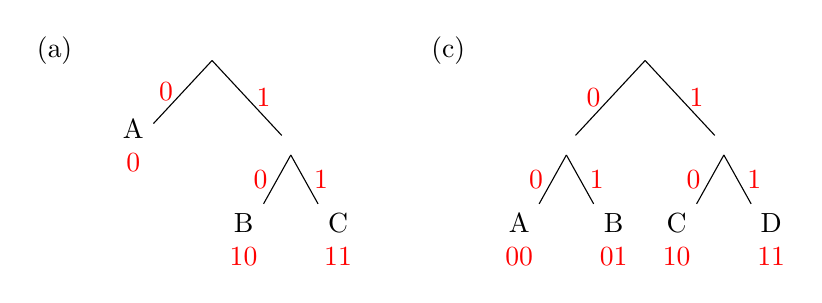
\begin{tikzpicture}[level distance=12mm, level 1/.style={sibling distance=20mm}, level 2/.style={sibling distance=12mm},
					edge from parent path={(\tikzparentnode.south) -- (\tikzchildnode)}]
				\tikzstyle{n} = [align=center]
				\tikzstyle{r} = [text=red]
				\node at (0,0) {(a)};
				\node at (2,0) {}
				child {node[n] {A\\\textcolor{red}{0}} edge from parent node[left,r] {0}}
				child {node {}
						child {node[n] {B\\\textcolor{red}{10}} edge from parent node[left,r] {0}}
						child {node[n] {C\\\textcolor{red}{11}} edge from parent node[right,r] {1}}
						edge from parent node[right,r] {1}};
				\node at (5,0) {(c)};
				\node at (7.5,0) {}
				child {node {}
						child {node[n] {A\\\textcolor{red}{00}} edge from parent node[left,r] {0}}
						child {node[n] {B\\\textcolor{red}{01}} edge from parent node[right,r] {1}}
						edge from parent node[left,r] {0}}
				child {node {}
						child {node[n] {C\\\textcolor{red}{10}} edge from parent node[left,r] {0}}
						child {node[n] {D\\\textcolor{red}{11}} edge from parent node[right,r] {1}}
						edge from parent node[right,r] {1}};
			\end{tikzpicture}
		\end{figure}
	\end{myanswer}
\end{myexercise}

\begin{myexercise}\label{ex:haeufigkeiten}
	Gegeben ist der Text \texttt{ANANASSAFT}.
	\begin{aenum}
		\item Bestimmen Sie die absolute und die relative Häufigkeit jedes Buchstabens.
		\item Wie viele Bits braucht der Text mit einer Kodierung, bei der alle Buchstaben gleich viele Bits haben?
	\end{aenum}
	\begin{myanswer}
		\begin{aenum}
			\item Der Text hat 10 Buchstaben.
			      \begin{center}
				      \begin{tabular}{cccccc}
					      Buchstabe           & A    & N    & S    & F    & T    \\\midrule
					      Absolute Häufigkeit & 4    & 2    & 2    & 1    & 1    \\
					      Relative Häufigkeit & 40\% & 20\% & 20\% & 10\% & 10\%
				      \end{tabular}
			      \end{center}
			\item Es kommen 5 verschiedene Buchstaben vor. 2 Bits reichen nur für $2^2=4$ Buchstaben, mit 3 Bits gibt es $2^3=8$ Möglichkeiten. Jeder Buchstabe braucht also 3 Bits, der ganze Text $10\times3=30$ Bits.
		\end{aenum}
	\end{myanswer}
\end{myexercise}

\begin{myexercise}
	Wir haben einen Text mit 100 Buchstaben und den Buchstaben A, B, C, D sowie E. Im Text kommt A 55-mal, D und E jeweils 20-mal, B 3-mal und C 2-mal vor. Wählen Sie eine präfixfreie Kodierung der 5 Buchstaben des Alphabets, sodass die resultierende binäre Darstellung des Textes so kurz wie möglich wird.
	\begin{enumerate}
		\item Visualisieren Sie den Prozess bei der Wahl der Kodierungen der einzelnen Buchstaben mit einem Baumdiagramm.
		\item  Wie lang ist die binäre Darstellung des Texts mit Ihrer Kodierung?
	\end{enumerate}
	\begin{myanswer}
		Eine mögliche Lösung:
		\begin{figure}[H]
			\centering
			\begin{tikzpicture}
				[-,>=stealth',
					level distance=18mm,
					level 1/.style={sibling distance=60mm},
					level 2/.style={sibling distance=30mm},
					level 3/.style={sibling distance=15mm},
					level 4/.style={sibling distance=12mm},
					leaf/.style={circle, draw},
					label/.style={red},
					edge from parent path={(\tikzparentnode.south) -- (\tikzchildnode)}]


				\usetikzlibrary{shapes}
				\tikzstyle{n} = [align=center]
				\tikzstyle{r} = [text=red]

				\node[n]{\textcolor{RoyalBlue}{A,B,C,D,E}\\ 100\%}[edge from parent]
				child {node[n] {\textcolor{RoyalBlue}{A}\\ 55\%\\\textcolor{red}{0}}
						edge from parent node[left,r]{0};
					}
				child {node[n]{\textcolor{RoyalBlue}{B,C,D,E}\\ 45\%}
						child {node[n] {\textcolor{RoyalBlue}{D}\\ 20\%\\\textcolor{red}{10}}
								edge from parent[] node[left,r]{0};
							}
						child {node[n] {\textcolor{RoyalBlue}{B,C,E}\\ 25\%}
								child {node[n] {\textcolor{RoyalBlue}{E}\\20\%\\\textcolor{red}{110}}
										edge from parent[] node[left,r]{0};
									}
								child {node[n] {\textcolor{RoyalBlue}{B,C}\\ 5\%}
										child {node[n] {\textcolor{RoyalBlue}{B}\\3\%\\\textcolor{red}{1110}}
												edge from parent[] node[left,r]{0};
											}
										child {node[n] {\textcolor{RoyalBlue}{C}\\ 2\%\\\textcolor{red}{1111}}
												edge from parent[] node[r,right]{1};
											}
										edge from parent[] node[r,right]{1};
									}
								edge from parent[] node[r,right]{1};
							}
						edge from parent node[r,right]{1};
					};
			\end{tikzpicture}
		\end{figure}
		Die Länge des gesamten Texts berechnet sich aus der Summe der Häufigkeiten der Buchstaben mal deren Kodierungslänge:
		\begin{table}[H]
			\centering
			\begin{tabular}{ccc}
				Buchstabe & Kodierung & Länge der Kodierung \\\midrule
				A         & 0         & 1                   \\
				B         & 1110      & 4                   \\
				C         & 1111      & 4                   \\
				D         & 10        & 2                   \\
				E         & 110       & 3
			\end{tabular}
		\end{table}
		\[55\times1+3\times4 + 2\times4 + 20\times2 + 20\times3 = 175\]
	\end{myanswer}
\end{myexercise}

\subsection{Top-Down-Ansatz: Maximale Balance}
\textbf{Idee}: Summe der Buchstabenhäufigkeiten im linken und rechten Teilbaum ausbalancieren.

\textbf{Regel}: Die Buchstaben werden in zwei Gruppen geteilt, deren Häufigkeiten zusammen möglichst gleich gross sind. Die Gruppen dürfen beliebige Buchstaben enthalten, diese müssen nicht nebeneinander in der Tabelle stehen. Gewählt wird die Teilung mit der kleinsten Differenz. Haben mehrere Teilungen dieselbe kleinste Differenz, darf man jede davon nehmen. Die linke Gruppe erhält die Ziffer 0, die rechte die Ziffer 1. Jede Gruppe mit mehr als einem Buchstaben wird auf dieselbe Weise weiter geteilt.

\begin{table}[H]
	\centering
	\begin{tabular}{ccccccc}
		\textbf{Buchstabe}  & \textbf{A} & \textbf{B} & \textbf{C} & \textbf{D} & \textbf{E} & \textbf{F} \\\midrule
		Relative Häufigkeit & 25\%       & 25\%       & 13\%       & 13\%       & 12\%       & 12\%
	\end{tabular}
	\caption{Beispiel-Häufigkeiten von Buchstaben}
	\label{table:ex-topdown}
\end{table}

\begin{figure}[H]
	\centering
	\begin{subfigure}{.49\textwidth}
		\centering
		\begin{tikzpicture}
			[-,>=stealth',
				level distance=18mm,
				level 1/.style={sibling distance=30mm},
				level 2/.style={sibling distance=30mm},
				level 3/.style={sibling distance=15mm},
				level 4/.style={sibling distance=12mm},
				leaf/.style={circle, draw},
				label/.style={red},
				edge from parent path={(\tikzparentnode.south) -- (\tikzchildnode)},
				background rectangle/.style={fill=black!3,rounded corners},
				show background rectangle]


			\usetikzlibrary{shapes}
			\tikzstyle{n} = [align=center]
			\tikzstyle{r} = [text=red]

			\node[n]{\textcolor{RoyalBlue}{A,B,C,D,E,F}\\ 100\%}[edge from parent]
			child {node[n] {\textcolor{RoyalBlue}{A,B}\\ 50\%}
					edge from parent node[left,r]{0};
				}
			child {node[n]{\textcolor{RoyalBlue}{C,D,E,F}\\ 50\%}
					edge from parent node[r,right]{1};
				};
		\end{tikzpicture}
		\caption{Schritt 1}
	\end{subfigure}
	\hfill
	\begin{subfigure}{.49\textwidth}
		\centering
		\begin{tikzpicture}
			[-,>=stealth',
				level distance=18mm,
				level 1/.style={sibling distance=30mm},
				level 2/.style={sibling distance=30mm},
				level 3/.style={sibling distance=15mm},
				level 4/.style={sibling distance=12mm},
				leaf/.style={circle, draw},
				label/.style={red},
				edge from parent path={(\tikzparentnode.south) -- (\tikzchildnode)},background rectangle/.style={fill=black!3,rounded corners}, show background rectangle]


			\usetikzlibrary{shapes}
			\tikzstyle{n} = [align=center]
			\tikzstyle{r} = [text=red]

			\node[n]{\textcolor{RoyalBlue}{A,B,C,D,E,F}\\ 100\%}[edge from parent]
			child {node[n] {\textcolor{RoyalBlue}{A,B}\\ 50\%}
					child {node[n] {\textcolor{RoyalBlue}{A}\\ 25\%\\\textcolor{red}{00}}
							edge from parent[] node[left,r]{0};
						}
					child {node[n] {\textcolor{RoyalBlue}{B}\\ 25\%\\\textcolor{red}{01}}
							edge from parent[] node[r,right]{1};
						}
					edge from parent node[left,r]{0};
				}
			child {node[n]{\textcolor{RoyalBlue}{C,D,E,F}\\ 50\%}
					edge from parent node[r,right]{1};
				};
		\end{tikzpicture}
		\caption{Schritt 2}
	\end{subfigure}
	\begin{subfigure}{\textwidth}
		\centering
		\begin{tikzpicture}
			[-,>=stealth',
				level distance=18mm,
				level 1/.style={sibling distance=60mm},
				level 2/.style={sibling distance=30mm},
				level 3/.style={sibling distance=15mm},
				level 4/.style={sibling distance=12mm},
				leaf/.style={circle, draw},
				label/.style={red},
				edge from parent path={(\tikzparentnode.south) -- (\tikzchildnode)},background rectangle/.style={fill=black!3,rounded corners}, show background rectangle]


			\usetikzlibrary{shapes}
			\tikzstyle{n} = [align=center]
			\tikzstyle{r} = [text=red]

			\node[n]{\textcolor{RoyalBlue}{A,B,C,D,E,F}\\ 100\%}[edge from parent]
			child {node[n] {\textcolor{RoyalBlue}{A,B}\\ 50\%}
					child {node[n] {\textcolor{RoyalBlue}{A}\\ 25\%\\\textcolor{red}{00}}
							edge from parent[] node[left,r]{0};
						}
					child {node[n] {\textcolor{RoyalBlue}{B}\\ 25\%\\\textcolor{red}{01}}
							edge from parent[] node[r,right]{1};
						}
					edge from parent node[left,r]{0};
				}
			child {node[n]{\textcolor{RoyalBlue}{C,D,E,F}\\ 50\%}
					child {node[n] {\textcolor{RoyalBlue}{C,E}\\ 25\%}
							edge from parent[] node[left,r]{0};
						}
					child {node[n] {\textcolor{RoyalBlue}{D,F}\\ 25\%}
							edge from parent[] node[r,right]{1};
						}
					edge from parent node[r,right]{1};
				};
		\end{tikzpicture}
		\caption{Schritt 3}
	\end{subfigure}

	\begin{subfigure}{\textwidth}
		\centering
		\begin{tikzpicture}
			[-,>=stealth',
				level distance=18mm,
				level 1/.style={sibling distance=60mm},
				level 2/.style={sibling distance=30mm},
				level 3/.style={sibling distance=15mm},
				level 4/.style={sibling distance=12mm},
				leaf/.style={circle, draw},
				label/.style={red},
				edge from parent path={(\tikzparentnode.south) -- (\tikzchildnode)},background rectangle/.style={fill=black!3,rounded corners}, show background rectangle]


			\usetikzlibrary{shapes}
			\tikzstyle{n} = [align=center]
			\tikzstyle{r} = [text=red]

			\node[n]{\textcolor{RoyalBlue}{A,B,C,D,E,F}\\ 100\%}[edge from parent]
			child {node[n] {\textcolor{RoyalBlue}{A,B}\\ 50\%}
					child {node[n] {\textcolor{RoyalBlue}{A}\\ 25\%\\\textcolor{red}{00}}
							edge from parent[] node[left,r]{0};
						}
					child {node[n] {\textcolor{RoyalBlue}{B}\\ 25\%\\\textcolor{red}{01}}
							edge from parent[] node[r,right]{1};
						}
					edge from parent node[left,r]{0};
				}
			child {node[n]{\textcolor{RoyalBlue}{C,D,E,F}\\ 50\%}
					child {node[n] {\textcolor{RoyalBlue}{C,E}\\ 25\%}
							child {node[n] {\textcolor{RoyalBlue}{C}\\ 13\%\\\textcolor{red}{100}}
									edge from parent[] node[left,r]{0};
								}
							child {node[n] {\textcolor{RoyalBlue}{E}\\ 12\%\\\textcolor{red}{101}}
									edge from parent[] node[r,right]{1};
								}
							edge from parent[] node[left,r]{0};
						}
					child {node[n] {\textcolor{RoyalBlue}{D,F}\\ 25\%}
							child {node[n] {\textcolor{RoyalBlue}{D}\\ 13\%\\\textcolor{red}{110}}
									edge from parent[] node[left,r]{0};
								}
							child {node[n] {\textcolor{RoyalBlue}{F}\\ 12\%\\\textcolor{red}{111}}
									edge from parent[] node[r,right]{1};
								}
							edge from parent[] node[r,right]{1};
						}
					edge from parent node[r,right]{1};
				};
		\end{tikzpicture}
		\caption{Schritt 4 (Kodierung)}
	\end{subfigure}
	\caption{Schritt-für-Schritt-Erstellung des Baumdiagramms für \cref{table:ex-topdown} mit dem \tib{Top-Down}-Ansatz.}
\end{figure}

\begin{myexercise}
	Nutzen Sie die Strategie der maximalen Balance, um die präfixfreien Kodierungen für Texte
	mit folgenden Buchstabenhäufigkeiten zu entwerfen.
	\begin{enumerate}
		\item A - 57\%, B - 23\%, C - 12\%, D - 8\%
		\item A - 25\%, B - 20\%, C - 14\%, D - 11\%, E - 10\%, F - 10\%, G - 5\%, H - 5\%
		\item A - 33\%, B - 30\%, C - 17\%, D - 14\%, E - 6\%
	\end{enumerate}

	\begin{myanswer}
		\begin{figure}[H]
			\centering
			\begin{tikzpicture}
				[-,>=stealth',
					level distance=18mm,
					level 1/.style={sibling distance=60mm},
					level 2/.style={sibling distance=30mm},
					level 3/.style={sibling distance=15mm},
					level 4/.style={sibling distance=12mm},
					leaf/.style={circle, draw},
					label/.style={red},
					edge from parent path={(\tikzparentnode.south) -- (\tikzchildnode)},background rectangle/.style={fill=black!3,rounded corners}, show background rectangle]


				\usetikzlibrary{shapes}
				\tikzstyle{n} = [align=center]
				\tikzstyle{r} = [text=red]

				\node[n]{\textcolor{RoyalBlue}{A,B,C,C}\\ 100\%}[edge from parent]
				child {node[n] {\textcolor{RoyalBlue}{A}\\ 57\%\\\textcolor{red}{0}}
						edge from parent node[left,r]{0};
					}
				child {node[n]{\textcolor{RoyalBlue}{B,C,C}\\ 43\%}
						child {node[n] {\textcolor{RoyalBlue}{C,C}\\ 20\%}
								child {node[n] {\textcolor{RoyalBlue}{C}\\ 12\%\\\textcolor{red}{100}}
										edge from parent[] node[left,r]{0};
									}
								child {node[n] {\textcolor{RoyalBlue}{C}\\ 8\%\\\textcolor{red}{101}}
										edge from parent[] node[r,right]{1};
									}
								edge from parent[] node[left,r]{0};
							}
						child {node[n] {\textcolor{RoyalBlue}{B}\\ 23\%\\\textcolor{red}{11}}
								edge from parent[] node[r,right]{1};
							}
						edge from parent node[r,right]{1};
					};
			\end{tikzpicture}
			\caption{Lösungsvorschlag für Teilaufgabe 1}
		\end{figure}
	\end{myanswer}

	\begin{myanswer}
		Für Teilaufgabe 2 gibt es mehrere Lösungsmöglichkeiten, z.B.:
		\begin{figure}[H]
			\centering
			\begin{tikzpicture}
				[-,>=stealth',
					level distance=18mm,
					level 1/.style={sibling distance=60mm},
					level 2/.style={sibling distance=30mm},
					level 3/.style={sibling distance=15mm},
					level 4/.style={sibling distance=12mm},
					leaf/.style={circle, draw},
					label/.style={red},
					edge from parent path={(\tikzparentnode.south) -- (\tikzchildnode)},background rectangle/.style={fill=black!3,rounded corners}, show background rectangle]


				\usetikzlibrary{shapes}
				\tikzstyle{n} = [align=center]
				\tikzstyle{r} = [text=red]

				\node[n]{\textcolor{RoyalBlue}{A,B,C,D,E,F,G,H}\\ 100\%}[edge from parent]
				child {node[n] {\textcolor{RoyalBlue}{A,C,D}\\ 50\%}
						child {node[n] {\textcolor{RoyalBlue}{A}\\ 25\%\\\textcolor{red}{00}}
								edge from parent[] node[left,r]{0};
							}
						child {node[n] {\textcolor{RoyalBlue}{C,D}\\ 25\%}
								child {node[n] {\textcolor{RoyalBlue}{C}\\ 14\%\\\textcolor{red}{010}}
										edge from parent[] node[left,r]{0};
									}
								child {node[n] {\textcolor{RoyalBlue}{D}\\ 11\%\\\textcolor{red}{011}}
										edge from parent[] node[r,right]{1};
									}
								edge from parent[] node[r,right]{1};
							}
						edge from parent node[left,r]{0};
					}
				child {node[n]{\textcolor{RoyalBlue}{B,E,F,G,H}\\ 50\%}
						child {node[n] {\textcolor{RoyalBlue}{B,G}\\ 25\%}
								child {node[n] {\textcolor{RoyalBlue}{B}\\ 20\%\\\textcolor{red}{100}}
										edge from parent[] node[left,r]{0};
									}
								child {node[n] {\textcolor{RoyalBlue}{G}\\ 5\%\\\textcolor{red}{101}}
										edge from parent[] node[r,right]{1};
									}
								edge from parent[] node[left,r]{0};
							}
						child {node[n] {\textcolor{RoyalBlue}{E,F,H}\\ 25\%}
								child {node[n] {\textcolor{RoyalBlue}{E,H}\\ 15\%}
										child {node[n] {\textcolor{RoyalBlue}{E}\\ 10\%\\\textcolor{red}{1100}}
												edge from parent[] node[left,r]{0};
											}
										child {node[n] {\textcolor{RoyalBlue}{H}\\ 5\%\\\textcolor{red}{1101}}
												edge from parent[] node[r,right]{1};
											}
										edge from parent[] node[left,r]{0};
									}
								child {node[n] {\textcolor{RoyalBlue}{F}\\ 10\%\\\textcolor{red}{111}}
										edge from parent[] node[r,right]{1};
									}
								edge from parent[] node[r,right]{1};
							}
						edge from parent node[r,right]{1};
					};
			\end{tikzpicture}
			\caption{Lösungsvorschlag für Teilaufgabe 2}
		\end{figure}
	\end{myanswer}

	\begin{myanswer}
		\begin{figure}[H]
			\centering
			\begin{tikzpicture}
				[-,>=stealth',
					level distance=18mm,
					level 1/.style={sibling distance=60mm},
					level 2/.style={sibling distance=30mm},
					level 3/.style={sibling distance=15mm},
					level 4/.style={sibling distance=12mm},
					leaf/.style={circle, draw},
					label/.style={red},
					edge from parent path={(\tikzparentnode.south) -- (\tikzchildnode)},background rectangle/.style={fill=black!3,rounded corners}, show background rectangle]


				\usetikzlibrary{shapes}
				\tikzstyle{n} = [align=center]
				\tikzstyle{r} = [text=red]

				\node[n]{\textcolor{RoyalBlue}{A,B,C,D,E}\\ 100\%}[edge from parent]
				child {node[n] {\textcolor{RoyalBlue}{A,C}\\ 50\%\\}
						child {node[n] {\textcolor{RoyalBlue}{A}\\ 33\%\\\textcolor{red}{00}}
								edge from parent[] node[left,r]{0};
							}
						child {node[n] {\textcolor{RoyalBlue}{C}\\ 17\%\\\textcolor{red}{01}}
								edge from parent[] node[r,right]{1};
							}
						edge from parent node[left,r]{0};
					}
				child {node[n]{\textcolor{RoyalBlue}{B,D,E}\\ 50\%}
						child {node[n] {\textcolor{RoyalBlue}{D,E}\\ 20\%}
								child {node[n] {\textcolor{RoyalBlue}{D}\\ 14\%\\\textcolor{red}{100}}
										edge from parent[] node[left,r]{0};
									}
								child {node[n] {\textcolor{RoyalBlue}{E}\\ 6\%\\\textcolor{red}{101}}
										edge from parent[] node[r,right]{1};
									}
								edge from parent[] node[left,r]{0};
							}
						child {node[n] {\textcolor{RoyalBlue}{B}\\ 30\%\\\textcolor{red}{11}}
								edge from parent[] node[r,right]{1};
							}
						edge from parent node[r,right]{1};
					};
			\end{tikzpicture}
			\caption{Lösungsvorschlag für Teilaufgabe 3}
		\end{figure}
	\end{myanswer}

\end{myexercise}

\begin{mychallenge}
	Schlagen Sie eine Häufigkeitsverteilung für Buchstaben so vor, dass die Strategie der maximalen Balance eindeutig ein Baumdiagramm bestimmt, in dem ein 10-mal häufigerer Buchstabe eine längere Kodierung hat als ein 10-mal seltener vorkommender Buchstabe.
	\begin{myanswer}
		Ein Beispiel: A -- 1\%, B -- 49\%, C -- 24\%, D -- 16\%, E -- 10\%.

		Die einzige Teilung mit Differenz 0 ist \{A,B\} (50\%) gegen \{C,D,E\} (50\%). \{A,B\} wird in A und B geteilt. Bei \{C,D,E\} hat die Teilung C (24\%) gegen \{D,E\} (26\%) die kleinste Differenz. Bis auf das Vertauschen von links und rechts entsteht also nur ein Baum, zum Beispiel mit der Kodierung
		\[\text{A} = \texttt{00},\quad \text{B} = \texttt{01},\quad \text{C} = \texttt{10},\quad \text{D} = \texttt{110},\quad \text{E} = \texttt{111}.\]
		E kommt zehnmal häufiger vor als A, erhält aber 3 Bits statt 2.
	\end{myanswer}
\end{mychallenge}

\begin{myexercise}\label{ex:problem}
	\textbf{Problem}: Was passiert bei folgender Verteilung?
	\begin{table}[H]
		\centering
		\begin{tabular}{ccccccc}
			\textbf{Buchstabe}  & \textbf{A} & \textbf{B} & \textbf{C} & \textbf{D} & \textbf{E} & \textbf{F} \\\midrule
			Relative Häufigkeit & 49\%       & 1\%        & 25\%       & 8\%        & 9\%        & 8\%
		\end{tabular}
	\end{table}


	\begin{myanswer}
		\begin{figure}[H]
			\centering
			\begin{tikzpicture}
				[-,>=stealth',
					level distance=15mm,
					level 1/.style={sibling distance=60mm},
					level 2/.style={sibling distance=30mm},
					level 3/.style={sibling distance=15mm},
					level 4/.style={sibling distance=15mm},
					level 5/.style={sibling distance=15mm},
					leaf/.style={circle, draw},
					label/.style={red},
					edge from parent path={(\tikzparentnode.south) -- (\tikzchildnode)},background rectangle/.style={fill=black!3,rounded corners}, show background rectangle]


				\usetikzlibrary{shapes}
				\tikzstyle{n} = [align=center]
				\tikzstyle{r} = [text=red]

				\node[n]{\textcolor{RoyalBlue}{A,B,C,D,E,F}\\ 100\%}[edge from parent]
				child {node[n] {\textcolor{RoyalBlue}{A,B}\\ 50\%}
						child {node[n] {\textcolor{RoyalBlue}{A}\\49\%\\\textcolor{red}{00}}
								edge from parent[] node[left,r]{0};
							}
						child {node[n, draw] {\textcolor{RoyalBlue}{B}\\ 1\%\\\textcolor{red}{01}}
								edge from parent[] node[r,right]{1};
							}
						edge from parent node[left,r]{0};
					}
				child {node[n]{\textcolor{RoyalBlue}{C,D,E,F}\\ 50\%}
						child {node[n] {\textcolor{RoyalBlue}{C}\\ 25\%\\\textcolor{red}{10}}
								edge from parent[] node[left,r]{0};
							}
						child {node[n] {\textcolor{RoyalBlue}{D,E,F}\\ 25\%}
								child {node[n, draw] {\textcolor{RoyalBlue}{E}\\ 9\%\\\textcolor{red}{110}}
										edge from parent[] node[left,r]{0};
									}
								child {node[n] {\textcolor{RoyalBlue}{D,F}\\ 16\%}
										child {node[n, draw] {\textcolor{RoyalBlue}{D}\\ 8\%\\\textcolor{red}{1110}}
												edge from parent[] node[left,r]{0};
											}
										child {node[n, draw] {\textcolor{RoyalBlue}{F}\\ 8\%\\\textcolor{red}{1111}}
												edge from parent[] node[right,r]{1};
											}
										edge from parent[] node[r,right]{1};
									}
								edge from parent[] node[r,right]{1};
							}
						edge from parent node[r,right]{1};
					};
			\end{tikzpicture}
		\end{figure}
		Wie wir sehen, wird der resultierende Baum nicht ausgeglichen: während der Buchstabe \enquote{D} (8\% Häufigkeit im Originaltext) beispielsweise mit \enquote{1110} kodiert wird, wird der Buchstabe \enquote{B} (1\% Häufigkeit im Originaltext) mit \enquote{01} kodiert, also mit einer kürzeren Bitfolge. Wie wir allerdings gesehen haben, sollten Buchstaben mit höherer Häufigkeit kürzer kodiert werden, da wir sie ja häufiger kodieren müssen und mit einer kürzeren Kodierungslänge somit insgesamt mehr Speicherplatz sparen.
	\end{myanswer}

\end{myexercise}
\subsection{Bottom-Up-Ansatz: Huffman-Kodierung}\label{sec:huffman}

Idee:
\begin{itemize}
	\item Jeder Buchstabe wird als Graph mit einem Knoten (=Baum mit einem Blatt) betrachtet. Die Häufigkeit jedes Buchstabens wird neben dem Blatt notiert. Wir wollen nun die Buchstaben zu Teilbäumen verbinden, bis wir einen einzigen Baum haben.
	      \begin{figure}[H]
		      \centering
		      \begin{tikzpicture}[background rectangle/.style={fill=black!3,rounded corners}, show background rectangle]
			      \tikzstyle{n} = [text width=1cm,align=center, draw, shape=circle]
			      \node[circle,draw, label={[align=center]below:\textcolor{RoyalBlue}{A}\\49\%}, ](a){};
			      \node[circle,draw, label={[align=center]below:\textcolor{RoyalBlue}{B}\\ 1\%}, right of=a](b){};
			      \node[circle,draw, label={[align=center]below:\textcolor{RoyalBlue}{C}\\ 25\%}, right of=b](c){};
			      \node[circle,draw, label={[align=center]below:\textcolor{RoyalBlue}{D}\\ 8\%}, right of=c](d){};
			      \node[circle,draw, label={[align=center]below:\textcolor{RoyalBlue}{E}\\ 9\%}, right of=d](e){};
			      \node[circle,draw, label={[align=center]below:\textcolor{RoyalBlue}{F}\\ 8\%}, right of=e](f){};
		      \end{tikzpicture}
		      \caption{Beispiel-Häufigkeiten von Buchstaben}
		      \label{fig:exFreqHuffman}
	      \end{figure}
	\item In einer Schleife: Wir schauen alle isolierten Blätter und Wurzeln von Teilbäumen an. Die beiden Knoten mit den kleinsten Prozentzahlen werden miteinander verbunden. Die neue Wurzel wird markiert mit dem Prozentsatz beider Knoten.
	      \begin{figure}[H]
		      \centering
		      \begin{tikzpicture}[-,>=stealth',
				      level distance=12mm,
				      level 1/.style={sibling distance=15mm},
				      level 2/.style={sibling distance=30mm},
				      level 3/.style={sibling distance=15mm},
				      level 4/.style={sibling distance=15mm},
				      level 5/.style={sibling distance=15mm},
				      leaf/.style={circle, draw},
				      edge from parent path={(\tikzparentnode.south) -- (\tikzchildnode)},background rectangle/.style={fill=black!3,rounded corners}, show background rectangle]


			      \usetikzlibrary{shapes}
			      \tikzstyle{n} = [align=center]
			      \tikzstyle{r} = [text=red]

			      \node[n]{\textcolor{RoyalBlue}{B,D}\\ 9\%}[edge from parent]
			      child {node[n] {\textcolor{RoyalBlue}{B}\\ 1\%}
					      edge from parent node[left,r]{};
				      }
			      child {node[n]{\textcolor{RoyalBlue}{D}\\ 8\%}
					      edge from parent node[r,right]{};
				      };
		      \end{tikzpicture}
		      \caption{Erster Schritt im Huffman-Kodierungs-Algorithmus}
	      \end{figure}
	\item Haben mehrere Knoten dieselbe kleinste Häufigkeit, darf man frei wählen: Die Länge des kodierten Texts ist bei jeder Wahl gleich. Wir verwenden die Konvention, den Teilbaum mit der geringsten Tiefe zu nehmen. So bleibt der Baum möglichst flach, und die längsten Codewörter werden nicht unnötig lang. Ganz eindeutig wird der Baum dadurch nicht: Im ersten Schritt darf B (1\%) mit D oder mit F verbunden werden, denn beide haben 8\% und sind einzelne Blätter.
\end{itemize}
\textbf{Welche Knoten werden als nächstes miteinander verbunden?}

\begin{figure}[H]
	\centering
	\begin{subfigure}{.45\textwidth}
		\begin{tikzpicture}[-,>=stealth',
				level distance=12mm,
				level 1/.style={sibling distance=15mm},
				level 2/.style={sibling distance=30mm},
				level 3/.style={sibling distance=15mm},
				level 4/.style={sibling distance=15mm},
				level 5/.style={sibling distance=15mm},
				leaf/.style={circle, draw},
				edge from parent path={(\tikzparentnode.south) -- (\tikzchildnode)},background rectangle/.style={fill=black!3,rounded corners}, show background rectangle]


			\usetikzlibrary{shapes}
			\tikzstyle{n} = [align=center]
			\tikzstyle{r} = [text=red]

			\node[n]{\textcolor{RoyalBlue}{B,D}\\ 9\%}[edge from parent]
			child {node[n] (b){\textcolor{RoyalBlue}{B}\\ 1\%}
					edge from parent node[left,r]{};
				}
			child {node[n]{\textcolor{RoyalBlue}{D}\\ 8\%}
					edge from parent node[r,right]{};
				};
			\node[n, left of=b](e){\textcolor{RoyalBlue}{E}\\ 9\%};
			\node[n, left of=e](f){\textcolor{RoyalBlue}{F}\\8\%};
			\node[n, left of=f](c){\textcolor{RoyalBlue}{C}\\ 25\%};
			\node[n, left of=c](a){\textcolor{RoyalBlue}{A}\\49\%};
		\end{tikzpicture}
		\caption{Schritt 1}
	\end{subfigure}\hfill
	\begin{subfigure}{.45\textwidth}
		\begin{tikzpicture}[-,>=stealth',
				level distance=15mm,
				level 1/.style={sibling distance=15mm},
				level 2/.style={sibling distance=30mm},
				level 3/.style={sibling distance=15mm},
				level 4/.style={sibling distance=15mm},
				level 5/.style={sibling distance=15mm},
				leaf/.style={circle, draw},
				edge from parent path={(\tikzparentnode.south) -- (\tikzchildnode)},background rectangle/.style={fill=black!3,rounded corners}, show background rectangle]


			\usetikzlibrary{shapes}
			\tikzstyle{n} = [align=center]
			\tikzstyle{r} = [text=red]

			\node(bd)[n]{\textcolor{RoyalBlue}{B,D}\\ 9\%}[edge from parent]
			child {node(b)[n] {\textcolor{RoyalBlue}{B}\\ 1\%}
					edge from parent node[left,r]{} ;
				}
			child {node[n]{\textcolor{RoyalBlue}{D}\\ 8\%}
					edge from parent node[r,right]{};
				};
			\node(ef)[n, left of=bd,xshift=-15mm]{\textcolor{RoyalBlue}{E,F}\\ 17\%}[edge from parent]
			child {node(f)[n] {\textcolor{RoyalBlue}{F}\\ 8\%}
					edge from parent node[left,r]{} ;
				}
			child {node[n]{\textcolor{RoyalBlue}{E}\\ 9\%}
					edge from parent node[r,right]{};
				};
			\node[n, left of=f](c){\textcolor{RoyalBlue}{C}\\ 25\%};
			\node[n, left of=c](a){\textcolor{RoyalBlue}{A}\\49\%};
		\end{tikzpicture}
		\caption{Schritt 2}
	\end{subfigure}\hfill
	\begin{subfigure}{.49\textwidth}
		\begin{tikzpicture}[-,>=stealth',
				level distance=15mm,
				level 1/.style={sibling distance=30mm},
				level 2/.style={sibling distance=15mm},
				level 3/.style={sibling distance=15mm},
				level 4/.style={sibling distance=15mm},
				level 5/.style={sibling distance=15mm},
				leaf/.style={circle, draw},
				edge from parent path={(\tikzparentnode.south) -- (\tikzchildnode)},background rectangle/.style={fill=black!3,rounded corners}, show background rectangle]

			\usetikzlibrary{shapes}
			\tikzstyle{n} = [align=center]
			\tikzstyle{r} = [text=red]

			\node(febd)[n]{\textcolor{RoyalBlue}{F,E,B,D}\\ 26\%}[edge from parent]
			child{node(ef)[n]{\textcolor{RoyalBlue}{E,F}\\ 17\%}
					child {node(f)[n] {\textcolor{RoyalBlue}{F}\\ 8\%}
							edge from parent node[left,r]{} ;
						}
					child {node[n]{\textcolor{RoyalBlue}{E}\\ 9\%}
							edge from parent node[r,right]{};
						}
					edge from parent node[r,right]{};
				}
			child{node(bd)[n]{\textcolor{RoyalBlue}{B,D}\\ 9\%}
					child {node(b)[n] {\textcolor{RoyalBlue}{B}\\ 1\%}
							edge from parent node[left,r]{} ;
						}
					child {node[n]{\textcolor{RoyalBlue}{D}\\ 8\%}
							edge from parent node[r,right]{};
						}
					edge from parent node[r,left]{};
				};
			\node[n, left of=f](c){\textcolor{RoyalBlue}{C}\\ 25\%};
			\node[n, left of=c](a){\textcolor{RoyalBlue}{A}\\49\%};
		\end{tikzpicture}
		\caption{Schritt 3}
	\end{subfigure}
	\begin{subfigure}{.49\textwidth}
		\begin{tikzpicture}[-,>=stealth',
				level distance=15mm,
				level 1/.style={sibling distance=20mm},
				level 2/.style={sibling distance=30mm},
				level 3/.style={sibling distance=15mm},
				level 4/.style={sibling distance=15mm},
				level 5/.style={sibling distance=15mm},
				leaf/.style={circle, draw},
				edge from parent path={(\tikzparentnode.south) -- (\tikzchildnode)},background rectangle/.style={fill=black!3,rounded corners}, show background rectangle]

			\usetikzlibrary{shapes}
			\tikzstyle{n} = [align=center]
			\tikzstyle{r} = [text=red]

			\node(cfebd)[n]{\textcolor{RoyalBlue}{C,F,E,B,D}\\ 51\%}[edge from parent]
			child{node(c)[n]{\textcolor{RoyalBlue}{C}\\ 25\%}
					edge from parent node[left,r]{} ;
				}
			child{node(febd)[n]{\textcolor{RoyalBlue}{F,E,B,D}\\ 26\%}
					child{node(ef)[n]{\textcolor{RoyalBlue}{E,F}\\ 17\%}
							child {node(f)[n] {\textcolor{RoyalBlue}{F}\\ 8\%}
									edge from parent node[left,r]{} ;
								}
							child {node[n]{\textcolor{RoyalBlue}{E}\\ 9\%}
									edge from parent node[r,right]{};
								}
							edge from parent node[r,right]{};
						}
					child{node(bd)[n]{\textcolor{RoyalBlue}{B,D}\\ 9\%}
							child {node(b)[n] {\textcolor{RoyalBlue}{B}\\ 1\%}
									edge from parent node[left,r]{} ;
								}
							child {node[n]{\textcolor{RoyalBlue}{D}\\ 8\%}
									edge from parent node[r,right]{};
								}
							edge from parent node[r,left]{};
						}
					edge from parent node[right,r]{};
				};
			\node[n, left=5mm of f](a){\textcolor{RoyalBlue}{A}\\49\%};
		\end{tikzpicture}
		\caption{Schritt 4}
	\end{subfigure}
	\hfill
	\begin{subfigure}{.49\textwidth}
		\begin{tikzpicture}[-,>=stealth',
				level distance=15mm,
				level 1/.style={sibling distance=20mm},
				level 2/.style={sibling distance=20mm},
				level 3/.style={sibling distance=30mm},
				level 4/.style={sibling distance=15mm},
				level 5/.style={sibling distance=15mm},
				leaf/.style={circle, draw},
				edge from parent path={(\tikzparentnode.south) -- (\tikzchildnode)},background rectangle/.style={fill=black!3,rounded corners}, show background rectangle]

			\usetikzlibrary{shapes}
			\tikzstyle{n} = [align=center]
			\tikzstyle{r} = [text=red]

			\node(acebd)[n]{\textcolor{RoyalBlue}{A,C,F,E,B,D}\\ 100\%}[edge from parent]
			child{node(a)[n]{\textcolor{RoyalBlue}{A}\\49\%}
					edge from parent node[left,r]{} ;
				}
			child{node(cfebd)[n]{\textcolor{RoyalBlue}{C,F,E,B,D}\\ 51\%}
					child{node(c)[n]{\textcolor{RoyalBlue}{C}\\ 25\%}
							edge from parent node[left,r]{} ;
						}
					child{node(febd)[n]{\textcolor{RoyalBlue}{F,E,B,D}\\ 26\%}
							child{node(ef)[n]{\textcolor{RoyalBlue}{E,F}\\ 17\%}
									child {node(f)[n] {\textcolor{RoyalBlue}{F}\\ 8\%}
											edge from parent node[left,r]{} ;
										}
									child {node[n]{\textcolor{RoyalBlue}{E}\\ 9\%}
											edge from parent node[r,right]{};
										}
									edge from parent node[r,right]{};
								}
							child{node(bd)[n]{\textcolor{RoyalBlue}{B,D}\\ 9\%}
									child {node(b)[n] {\textcolor{RoyalBlue}{B}\\ 1\%}
											edge from parent node[left,r]{} ;
										}
									child {node[n]{\textcolor{RoyalBlue}{D}\\ 8\%}
											edge from parent node[r,right]{};
										}
									edge from parent node[r,left]{};
								}
							edge from parent node[right,r]{};
						}
					edge from parent node[right,r]{};
				};
		\end{tikzpicture}
		\caption{Schritt 5}
	\end{subfigure}\hfill
	\begin{subfigure}{.49\textwidth}
		\begin{tikzpicture}[-,>=stealth',
				level distance=15mm,
				level 1/.style={sibling distance=20mm},
				level 2/.style={sibling distance=20mm},
				level 3/.style={sibling distance=30mm},
				level 4/.style={sibling distance=15mm},
				level 5/.style={sibling distance=15mm},
				leaf/.style={circle, draw},
				edge from parent path={(\tikzparentnode.south) -- (\tikzchildnode)},background rectangle/.style={fill=black!3,rounded corners}, show background rectangle]

			\usetikzlibrary{shapes}
			\tikzstyle{n} = [align=center]
			\tikzstyle{r} = [text=red]

			\node(acebd)[n]{\textcolor{RoyalBlue}{A,C,F,E,B,D}\\ 100\%}[edge from parent]
			child{node(a)[n]{\textcolor{RoyalBlue}{A}\\49\%\\\textcolor{red}{0}}
					edge from parent node[left,r]{0} ;
				}
			child{node(cfebd)[n]{\textcolor{RoyalBlue}{C,F,E,B,D}\\ 51\%}
					child{node(c)[n]{\textcolor{RoyalBlue}{C}\\ 25\%\\\textcolor{red}{10}}
							edge from parent node[left,r]{0} ;
						}
					child{node(febd)[n]{\textcolor{RoyalBlue}{F,E,B,D}\\ 26\%}
							child{node(ef)[n]{\textcolor{RoyalBlue}{E,F}\\ 17\%}
									child {node(f)[n] {\textcolor{RoyalBlue}{F}\\ 8\%\\\textcolor{red}{1100}}
											edge from parent node[left,r]{0} ;
										}
									child {node[n]{\textcolor{RoyalBlue}{E}\\ 9\%\\\textcolor{red}{1101}}
											edge from parent node[r,right]{1};
										}
									edge from parent node[r,left]{0};
								}
							child{node(bd)[n]{\textcolor{RoyalBlue}{B,D}\\ 9\%}
									child {node(b)[n] {\textcolor{RoyalBlue}{B}\\ 1\%\\\textcolor{red}{1110}}
											edge from parent node[left,r]{0} ;
										}
									child {node[n]{\textcolor{RoyalBlue}{D}\\ 8\%\\\textcolor{red}{1111}}
											edge from parent node[r,right]{1};
										}
									edge from parent node[r,right]{1};
								}
							edge from parent node[right,r]{1};
						}
					edge from parent node[right,r]{1};
				};
		\end{tikzpicture}
		\caption{Schritt 6 (Kodierung)}
	\end{subfigure}
	\caption{Schritt-für-Schritt-Erstellung des Baumdiagramms für \cref{fig:exFreqHuffman} mit der \tib{Huffman}-Kodierung}
	\label{fig:huffman-schritte}
\end{figure}

\begin{myexercise}
	Weshalb haben wir in Schritt 2 einen Baum \{\textcolor{RoyalBlue}{E,F}\} statt \{\textcolor{RoyalBlue}{F,B,D}\} gemacht?
	\begin{myanswer}
		Nach Schritt 1 hat F mit 8\% die kleinste Häufigkeit. Danach folgen E und \{B,D\} mit je 9\%. F wird also mit einem dieser beiden Knoten verbunden. Nach der Gleichstandsregel nehmen wir den Teilbaum mit der geringsten Tiefe: E ist ein einzelnes Blatt (Tiefe 0), \{B,D\} hat bereits Tiefe 1.

		Mit \{F,B,D\} wäre der kodierte Text gleich lang, B und D bekämen aber Codewörter mit 5 statt 4 Bits.
	\end{myanswer}
\end{myexercise}

Um Kodierungen zu vergleichen, berechnet man die \tib{mittlere Codelänge} in Bit pro Zeichen: Man multipliziert die Länge jedes Codeworts mit der relativen Häufigkeit seines Buchstabens und addiert diese Produkte. Für die Verteilung aus \cref{fig:exFreqHuffman} ergibt sich:
\begin{itemize}
	\item Huffman-Kodierung (\cref{fig:huffman-schritte}): $0.49\times1 + 0.25\times2 + (0.08+0.09+0.01+0.08)\times4 = 2.03$ Bit pro Zeichen
	\item Maximale Balance (Lösung zu \cref{ex:problem}): $(0.49+0.01+0.25)\times2 + 0.09\times3 + (0.08+0.08)\times4 = 2.41$ Bit pro Zeichen
	\item Kodierung mit fester Länge: Für sechs Buchstaben braucht jeder Buchstabe 3 Bits, also 3 Bit pro Zeichen.
\end{itemize}
Ein Text mit 1000 Zeichen braucht mit Huffman also rund 2030 Bits, mit der maximalen Balance rund 2410 Bits und mit fester Länge 3000 Bits.

Als Fazit kann Folgendes festgehalten werden:
\begin{itemize}
	\item Strategie der \textbf{maximalen Balance}: \textit{top-down}-Ansatz (von Wurzel zu Blättern), kann zu suboptimalen Kodierungen führen
	\item \textbf{Huffman-Kodierung}: \textit{bottom-up}-Ansatz (von Blättern zur Wurzel), garantiert die kürzestmögliche Gesamtlänge des kodierten Texts (unter allen präfixfreien Kodierungen einzelner Buchstaben)
\end{itemize}

\begin{myexercise}
	Verwenden Sie den Algorithmus von Huffman, um präfixfreie Kodierungen für die folgenden Häufigkeitsverteilungen von Buchstaben zu konstruieren.
	\begin{itemize}
		\item A - 25\%, B - 25\%, C - 13\%, D - 12\%, E - 6\%, F - 7\%, G - 6\%, H - 6\%
		\item A - 15\%, B - 15\%, C - 15\%, D - 15\%, E - 15\%, F - 15\%, G - 10\%
		\item A - 45\%, B - 15\%, C - 7\%, D - 7\%, E - 6\%, F - 10\%, G - 10\%
		\item A - 33\%, B - 18\%, C - 18\%, D - 17\%, E - 4\%, F - 4\%, G - 3\%, H - 3\%
	\end{itemize}
	Vergleichen Sie in der Klasse die entstandenen präfixfreien Kodierungen. Die Lösungen
	zur jeweiligen Häufigkeitsverteilung dürfen sich unterscheiden. Wo liegen die Unterschiede
	und was haben die unterschiedlichen Lösungen immer gemeinsam?

	Bei welchen der vier Häufigkeitsverteilungen der Buchstaben werden Sie mit der Strategie
	der maximalen Balance gleich gute präfixfreie Kodierungen der Buchstaben erhalten wie mit der Huffman-Strategie und bei welchen nicht?
	Vergleichen Sie dazu die mittleren Codelängen.
	\begin{myanswer}
		Eine mögliche Lösung pro Verteilung, jeweils mit einer Kodierung der maximalen Balance zum Vergleich:
		\begin{center}
			\small
			\begin{tabular}{lcccccccc}
				\textbf{Verteilung 1} & A & B & C & D & E & F & G & H \\\midrule
				Häufigkeit & 25\% & 25\% & 13\% & 12\% & 6\% & 7\% & 6\% & 6\% \\
				Huffman & \texttt{01} & \texttt{10} & \texttt{110} & \texttt{000} & \texttt{0010} & \texttt{1111} & \texttt{0011} & \texttt{1110} \\
				Maximale Balance & \texttt{00} & \texttt{01} & \texttt{100} & \texttt{101} & \texttt{1100} & \texttt{1101} & \texttt{1110} & \texttt{1111}
			\end{tabular}
		\end{center}
		Mittlere Codelänge: Huffman 2.75, maximale Balance 2.75 Bit pro Zeichen.
		\begin{center}
			\small
			\begin{tabular}{lccccccc}
				\textbf{Verteilung 2} & A & B & C & D & E & F & G \\\midrule
				Häufigkeit & 15\% & 15\% & 15\% & 15\% & 15\% & 15\% & 10\% \\
				Huffman & \texttt{011} & \texttt{100} & \texttt{101} & \texttt{110} & \texttt{111} & \texttt{00} & \texttt{010} \\
				Maximale Balance & \texttt{00} & \texttt{010} & \texttt{011} & \texttt{100} & \texttt{101} & \texttt{110} & \texttt{111}
			\end{tabular}
		\end{center}
		Mittlere Codelänge: Huffman 2.85, maximale Balance 2.85 Bit pro Zeichen.
		\begin{center}
			\small
			\begin{tabular}{lccccccc}
				\textbf{Verteilung 3} & A & B & C & D & E & F & G \\\midrule
				Häufigkeit & 45\% & 15\% & 7\% & 7\% & 6\% & 10\% & 10\% \\
				Huffman & \texttt{0} & \texttt{110} & \texttt{1011} & \texttt{1110} & \texttt{1010} & \texttt{1111} & \texttt{100} \\
				Maximale Balance & \texttt{00} & \texttt{100} & \texttt{1100} & \texttt{1101} & \texttt{01} & \texttt{101} & \texttt{111}
			\end{tabular}
		\end{center}
		Mittlere Codelänge: Huffman 2.40, maximale Balance 2.63 Bit pro Zeichen.
		\begin{center}
			\small
			\begin{tabular}{lcccccccc}
				\textbf{Verteilung 4} & A & B & C & D & E & F & G & H \\\midrule
				Häufigkeit & 33\% & 18\% & 18\% & 17\% & 4\% & 4\% & 3\% & 3\% \\
				Huffman & \texttt{11} & \texttt{00} & \texttt{01} & \texttt{101} & \texttt{10010} & \texttt{10011} & \texttt{10000} & \texttt{10001} \\
				Maximale Balance & \texttt{00} & \texttt{100} & \texttt{110} & \texttt{01} & \texttt{1010} & \texttt{1110} & \texttt{1011} & \texttt{1111}
			\end{tabular}
		\end{center}
		Mittlere Codelänge: Huffman 2.59, maximale Balance 2.64 Bit pro Zeichen.

		Die Lösungen unterscheiden sich darin, welcher Ast die 0 und welcher die 1 erhält und wie bei gleichen Häufigkeiten gewählt wird. Dadurch ändern sich die Codewörter und manchmal auch die Längen einzelner Codewörter. Gemeinsam ist allen Huffman-Lösungen einer Verteilung die mittlere Codelänge und damit die Länge des kodierten Texts.

		Bei den Verteilungen 1 und 2 ist die maximale Balance gleich gut wie Huffman (2.75 bzw. 2.85 Bit pro Zeichen). Bei den Verteilungen 3 und 4 ist sie schlechter (2.63 statt 2.40 bzw. 2.64 statt 2.59 Bit pro Zeichen).
	\end{myanswer}
\end{myexercise}

\begin{myexercise}
	Komprimieren Sie das Wort \enquote{\texttt{ALLEMAL}} mit der Huffman-Kodierung. Wie lang ist der Text komprimiert? Wie lang wäre er mit einer Kodierung, bei der alle Buchstaben gleich viele Bits haben?
	\begin{myanswer}
		Wir beginnen damit, die Wortlänge zu zählen und die relativen Buchstabenhäufigkeiten zu bestimmen:
		\begin{itemize}
			\item Wortlänge: 7
			\item Buchstaben-Häufigkeiten: \texttt{A} - 2/7, \texttt{L} - 3/7, \texttt{E} - 1/7, \texttt{M} - 1/7
		\end{itemize}
		Nun können wir den Baum erstellen. Das Endergebnis könnte wie folgt aussehen:

		\begin{figure}[H]
			\centering
			\begin{tikzpicture}[-,>=stealth',
					level distance=15mm,
					level 1/.style={sibling distance=30mm},
					level 2/.style={sibling distance=15mm},
					level 3/.style={sibling distance=15mm},
					level 4/.style={sibling distance=15mm},
					level 5/.style={sibling distance=15mm},
					leaf/.style={circle, draw},
					edge from parent path={(\tikzparentnode.south) -- (\tikzchildnode)}]

				\usetikzlibrary{shapes}
				\tikzstyle{n} = [align=center]
				\tikzstyle{r} = [text=red]

				\node(febd)[n]{\textcolor{RoyalBlue}{A,L,E,M}\\ 7/7}
				child{node(ef)[n]{\textcolor{RoyalBlue}{A,E,M}\\ 4/7}
						child {node(f)[n] {\textcolor{RoyalBlue}{A}\\ 2/7}
								edge from parent node[r,left]{0} ;
							}
						child {node[n]{\textcolor{RoyalBlue}{E,M}\\ 2/7}
								child {node(f)[n] {\textcolor{RoyalBlue}{E}\\ 1/7}
										edge from parent node[r,left]{0} ;
									}
								child {node[n]{\textcolor{RoyalBlue}{M}\\ 1/7}
										edge from parent node[r,right]{1};
									}
								edge from parent node[r,right]{1};
							}
						edge from parent node[r,left]{0};
					}
				child{node(bd)[n]{\textcolor{RoyalBlue}{L}\\ 3/7}
						edge from parent node[r,right]{1};
					};
			\end{tikzpicture}
		\end{figure}

		Daraus ergibt sich folgende Kodierung für den Text \texttt{ALLEMAL}:
		\begin{itemize}
			\item \texttt{A: 00}
			\item \texttt{L: 1}
			\item \texttt{E: 010}
			\item \texttt{M: 011}
		\end{itemize}
		Der gesamte Text würde also wie folgt kodiert: \texttt{0011010011001} (13 Bits).

		Mit einer Kodierung fester Länge brauchen wir 2 Bits pro Buchstabe, da wir insgesamt 4 verschiedene Buchstaben (\texttt{A}, \texttt{L}, \texttt{E}, \texttt{M}) im Text haben und 2 Bits uns $2^2=4$ Möglichkeiten geben. Eine mögliche Kodierung wäre:

		\begin{itemize}
			\item \texttt{A: 00}
			\item \texttt{L: 01}
			\item \texttt{E: 11}
			\item \texttt{M: 10}
		\end{itemize}

		In diesem Fall würden wir 14 Bits für den Text benötigen. In diesem Beispiel haben wir durch die Kompression also nur ein Bit gespart. In anderen Fällen kann es jedoch viel mehr sein!
	\end{myanswer}
\end{myexercise}

\begin{myexercise}
	Klicken Sie auf \href{https://cmps-people.ok.ubc.ca/ylucet/DS/Huffman.html}{diesen Link}, um Huffman-Bäume Schritt für Schritt zu visualisieren.
\end{myexercise}

\subsection{So arbeitet ZIP: DEFLATE}\label{sec:deflate}
ZIP, gzip und PNG verwenden das Verfahren \tib{DEFLATE}. Es verbindet die beiden Ideen dieses Kapitels in zwei Stufen (\cref{fig:deflate}).

\begin{figure}[H]
	\centering
	\begin{tikzpicture}[node distance=.8cm,
			stufe/.style={draw, rounded corners, minimum height=.8cm, font=\bfseries},
			daten/.style={align=center, font=\small}]
		\node[daten] (text) {Text};
		\node[stufe, right=of text] (lz) {LZ77};
		\node[daten, right=of lz] (paare) {Zeichen\\und Paare};
		\node[stufe, right=of paare] (huff) {Huffman};
		\node[daten, right=of huff] (bits) {Bits};
		\draw[->] (text) -- (lz);
		\draw[->] (lz) -- (paare);
		\draw[->] (paare) -- (huff);
		\draw[->] (huff) -- (bits);
	\end{tikzpicture}
	\caption{DEFLATE in zwei Stufen}
	\label{fig:deflate}
\end{figure}

LZ77 ersetzt Wiederholungen durch Paare (Abstand, Länge). Was übrig bleibt, die einzelnen Zeichen und die Zahlen der Paare, kodiert DEFLATE anschliessend mit der Huffman-Kodierung aus \cref{sec:huffman}: Häufige Zeichen und häufige Längen erhalten kurze Codewörter. LZ77 nutzt aus, dass ganze Zeichenfolgen wiederkehren, Huffman, dass einzelne Zeichen unterschiedlich häufig sind.

Eine ZIP-Datei ist zudem ein Container. Für jede enthaltene Datei speichert sie Name, Datum, die komprimierten Daten und eine Prüfsumme (CRC-32). Damit erkennt das Programm beim Entpacken, ob die Daten beschädigt sind. Prüfsummen sind Thema im Skript Datenintegrität.

\begin{myexample}\label{ex:deflate-hallo}
	Der Text \texttt{HALLO HALLO HALLO} hat 17 Zeichen. Er wird hier mit allen Verfahren dieses Kapitels kodiert.

	\textbf{8 Bits pro Zeichen.} $17 \cdot 8 = 136$ Bits.

	\textbf{Feste Codelänge.} Der Text hat 5 verschiedene Zeichen (H, A, L, O, \textvisiblespace). 2 Bits reichen nur für 4 Zeichen, 3 Bits für $2^3 = 8$. Das ergibt $17 \cdot 3 = 51$ Bits.

	\textbf{Maximale Balance.} Die Häufigkeiten sind L~6, H~3, A~3, O~3, \textvisiblespace~2. Die Teilung \{L,H\} (9) gegen \{A,O,\textvisiblespace\} (8) ergibt L~\texttt{00}, H~\texttt{01}, A~\texttt{10}, O~\texttt{110}, \textvisiblespace~\texttt{111} und $6\cdot2 + 3\cdot2 + 3\cdot2 + 3\cdot3 + 2\cdot3 = 39$ Bits. Die Teilung \{L,\textvisiblespace\} (8) gegen \{H,A,O\} (9) hat dieselbe Differenz und ergibt 40 Bits.

	\textbf{Nur Huffman.} Huffman verbindet zuerst \textvisiblespace{} mit H (5, bei Gleichstand von H, A und O freie Wahl), dann A mit O (6), dann \{\textvisiblespace,H\} mit L (11, L hat bei Gleichstand mit \{A,O\} die geringere Tiefe) und am Schluss die beiden Teilbäume (\cref{fig:huffman-hallo}). Das ergibt A~\texttt{00}, O~\texttt{01}, L~\texttt{11}, \textvisiblespace~\texttt{100}, H~\texttt{101} und $3\cdot2 + 3\cdot2 + 6\cdot2 + 2\cdot3 + 3\cdot3 = 39$ Bits.
	\begin{figure}[H]
		\centering
		\begin{tikzpicture}[-,>=stealth',
				level distance=15mm,
				level 1/.style={sibling distance=60mm},
				level 2/.style={sibling distance=30mm},
				level 3/.style={sibling distance=15mm},
				edge from parent path={(\tikzparentnode.south) -- (\tikzchildnode)},
				background rectangle/.style={fill=black!3,rounded corners}, show background rectangle]
			\tikzstyle{n} = [align=center]
			\tikzstyle{r} = [text=red]
			\node[n]{\textcolor{RoyalBlue}{A,O,\textvisiblespace,H,L}\\ 17}
			child {node[n] {\textcolor{RoyalBlue}{A,O}\\ 6}
				child {node[n] {\textcolor{RoyalBlue}{A}\\ 3\\\textcolor{red}{00}}
					edge from parent node[left,r]{0}}
				child {node[n] {\textcolor{RoyalBlue}{O}\\ 3\\\textcolor{red}{01}}
					edge from parent node[right,r]{1}}
				edge from parent node[left,r]{0}}
			child {node[n] {\textcolor{RoyalBlue}{\textvisiblespace,H,L}\\ 11}
				child {node[n] {\textcolor{RoyalBlue}{\textvisiblespace,H}\\ 5}
					child {node[n] {\textcolor{RoyalBlue}{\textvisiblespace}\\ 2\\\textcolor{red}{100}}
						edge from parent node[left,r]{0}}
					child {node[n] {\textcolor{RoyalBlue}{H}\\ 3\\\textcolor{red}{101}}
						edge from parent node[right,r]{1}}
					edge from parent node[left,r]{0}}
				child {node[n] {\textcolor{RoyalBlue}{L}\\ 6\\\textcolor{red}{11}}
					edge from parent node[right,r]{1}}
				edge from parent node[right,r]{1}};
		\end{tikzpicture}
		\caption{Huffman-Baum für \texttt{HALLO HALLO HALLO}}
		\label{fig:huffman-hallo}
	\end{figure}

	\textbf{DEFLATE, Stufe 1: LZ77.} Ab dem 7.~Zeichen wiederholt sich alles, was 6 Zeichen weiter vorne steht, und zwar für die restlichen 11 Zeichen:
	\begin{center}
		\texttt{H A L L O \textvisiblespace{} (6,11)}
	\end{center}

	\textbf{DEFLATE, Stufe 2: Huffman.} Das Paar zählt als eigener Baustein \texttt{P}. Hinter seinem Codewort folgen Abstand und Länge mit je 5 Bits (5 Bits reichen für Zahlen bis 31; echtes DEFLATE kodiert auch diese Zahlen mit Huffman). Die 7 Bausteine haben die Häufigkeiten L~2 und H, A, O, \textvisiblespace, P je 1. Der Huffman-Algorithmus verbindet zuerst H mit A und O mit \textvisiblespace, dann P mit L (bei Gleichstand nach der geringsten Tiefe) und am Schluss die beiden Teilbäume (\cref{fig:deflate-hallo}).
	\begin{figure}[H]
		\centering
		\begin{tikzpicture}[-,>=stealth',
				level distance=15mm,
				level 1/.style={sibling distance=60mm},
				level 2/.style={sibling distance=30mm},
				level 3/.style={sibling distance=15mm},
				edge from parent path={(\tikzparentnode.south) -- (\tikzchildnode)},
				background rectangle/.style={fill=black!3,rounded corners}, show background rectangle]
			\tikzstyle{n} = [align=center]
			\tikzstyle{r} = [text=red]
			\node[n]{\textcolor{RoyalBlue}{P,L,H,A,O,\textvisiblespace}\\ 7}
			child {node[n] {\textcolor{RoyalBlue}{P,L}\\ 3}
				child {node[n] {\textcolor{RoyalBlue}{P}\\ 1\\\textcolor{red}{00}}
					edge from parent node[left,r]{0}}
				child {node[n] {\textcolor{RoyalBlue}{L}\\ 2\\\textcolor{red}{01}}
					edge from parent node[right,r]{1}}
				edge from parent node[left,r]{0}}
			child {node[n] {\textcolor{RoyalBlue}{H,A,O,\textvisiblespace}\\ 4}
				child {node[n] {\textcolor{RoyalBlue}{H,A}\\ 2}
					child {node[n] {\textcolor{RoyalBlue}{H}\\ 1\\\textcolor{red}{100}}
						edge from parent node[left,r]{0}}
					child {node[n] {\textcolor{RoyalBlue}{A}\\ 1\\\textcolor{red}{101}}
						edge from parent node[right,r]{1}}
					edge from parent node[left,r]{0}}
				child {node[n] {\textcolor{RoyalBlue}{O,\textvisiblespace}\\ 2}
					child {node[n] {\textcolor{RoyalBlue}{O}\\ 1\\\textcolor{red}{110}}
						edge from parent node[left,r]{0}}
					child {node[n] {\textcolor{RoyalBlue}{\textvisiblespace}\\ 1\\\textcolor{red}{111}}
						edge from parent node[right,r]{1}}
					edge from parent node[right,r]{1}}
				edge from parent node[right,r]{1}};
		\end{tikzpicture}
		\caption{Huffman-Baum der DEFLATE-Bausteine für \texttt{HALLO HALLO HALLO}}
		\label{fig:deflate-hallo}
	\end{figure}
	\begin{center}
		\begin{tabular}{lccr}
			\textbf{Baustein} & \textbf{Häufigkeit} & \textbf{Codewort} & \textbf{Bits} \\\midrule
			P & 1 & \texttt{00} & $1 \cdot 2 = 2$ \\
			L & 2 & \texttt{01} & $2 \cdot 2 = 4$ \\
			H & 1 & \texttt{100} & 3 \\
			A & 1 & \texttt{101} & 3 \\
			O & 1 & \texttt{110} & 3 \\
			\textvisiblespace & 1 & \texttt{111} & 3 \\\midrule
			\multicolumn{3}{l}{Summe Codewörter} & 18 \\
			\multicolumn{3}{l}{Abstand 6 und Länge 11, je 5 Bits} & 10 \\
			\multicolumn{3}{l}{\textbf{Total DEFLATE}} & \textbf{28}
		\end{tabular}
	\end{center}

	\textbf{Vergleich.} Als Ausgangspunkt dient die feste Codelänge mit 3 Bits pro Zeichen, die Ersparnis ist also $1 - \text{Bits}/51$ (\cref{table:vergleich-hallo}). Die Speicherung mit 8 Bits pro Zeichen steht nur in Klammern zum Vergleich.
	\begin{table}[H]
		\centering
		\begin{tabular}{lrr}
			\textbf{Verfahren} & \textbf{Bits} & \textbf{Ersparnis} \\\midrule
			(8 Bits pro Zeichen) & (136) & \\
			Feste Codelänge (3 Bits) & 51 & 0\% \\
			Maximale Balance & 39 & 23.5\% \\
			Huffman & 39 & 23.5\% \\
			DEFLATE (LZ77 und Huffman) & 28 & 45.1\%
		\end{tabular}
		\caption{Kodierungen von \texttt{HALLO HALLO HALLO} im Vergleich}
		\label{table:vergleich-hallo}
	\end{table}
\end{myexample}

\begin{myexercise}\label{ex:deflate-rose}
	Der Text \texttt{ROSE IST EINE ROSE IST EINE ROSE} hat 32 Zeichen (die Leerzeichen zählen mit). Gehen Sie vor wie in \cref{ex:deflate-hallo}.
	\begin{aenum}
		\item Wie viele Bits braucht der Text, wenn jedes Zeichen mit 8 Bits gespeichert wird?
		\item Wie viele Bits braucht er mit einer Kodierung fester Codelänge?
		\item Bestimmen Sie die Häufigkeiten der Zeichen. Zeichnen Sie das Baumdiagramm der maximalen Balance, geben Sie die Codewörter an und berechnen Sie die Anzahl Bits.
		\item Zeichnen Sie den Huffman-Baum, geben Sie die Codewörter an und berechnen Sie die Anzahl Bits.
		\item Kodieren Sie den Text mit LZ77.
		\item Wie in DEFLATE nehmen Sie das Paar als zusätzlichen Baustein \texttt{P} auf. Zeichnen Sie den Huffman-Baum der Bausteine. Hinter dem Codewort von \texttt{P} folgen Abstand und Länge mit je 5 Bits. Berechnen Sie die Anzahl Bits.
		\item Stellen Sie alle Verfahren in einer Tabelle mit der Anzahl Bits und der Ersparnis gegenüber der festen Codelänge zusammen.
	\end{aenum}
	\begin{myanswer}
		\begin{aenum}
			\item $32 \cdot 8 = 256$ Bits.
			\item Der Text hat 8 verschiedene Zeichen (R, O, S, E, I, T, N, \textvisiblespace). 3 Bits reichen ($2^3 = 8$), also $32 \cdot 3 = 96$ Bits.
			\item Häufigkeiten: E~7, \textvisiblespace~6, S~5, I~4, R~3, O~3, T~2, N~2. Die Teilung \{E,\textvisiblespace,R\} (16) gegen \{S,O,I,T,N\} (16) hat die Differenz 0. Danach werden E gegen \{\textvisiblespace,R\}, \{S,O\} gegen \{I,T,N\} und I gegen \{T,N\} geteilt (\cref{fig:maxbal-rose}).
			      \begin{figure}[H]
			      	\centering
			      	\begin{tikzpicture}[-,>=stealth', font=\small,
			      			level distance=13mm,
			      			level 1/.style={sibling distance=70mm},
			      			level 2/.style={sibling distance=36mm},
			      			level 3/.style={sibling distance=18mm},
			      			level 4/.style={sibling distance=14mm},
			      			edge from parent path={(\tikzparentnode.south) -- (\tikzchildnode)},
			      			background rectangle/.style={fill=black!3,rounded corners}, show background rectangle]
			      		\tikzstyle{n} = [align=center]
			      		\tikzstyle{r} = [text=red]
			      		\node[n]{\textcolor{RoyalBlue}{E,\textvisiblespace,R,S,O,I,T,N}\\ 32}
			      		child {node[n] {\textcolor{RoyalBlue}{E,\textvisiblespace,R}\\ 16}
			      			child {node[n] {\textcolor{RoyalBlue}{E}\\ 7\\\textcolor{red}{00}}
			      				edge from parent node[left,r]{0}}
			      			child {node[n] {\textcolor{RoyalBlue}{\textvisiblespace,R}\\ 9}
			      				child {node[n] {\textcolor{RoyalBlue}{\textvisiblespace}\\ 6\\\textcolor{red}{010}}
			      					edge from parent node[left,r]{0}}
			      				child {node[n] {\textcolor{RoyalBlue}{R}\\ 3\\\textcolor{red}{011}}
			      					edge from parent node[right,r]{1}}
			      				edge from parent node[right,r]{1}}
			      			edge from parent node[left,r]{0}}
			      		child {node[n] {\textcolor{RoyalBlue}{S,O,I,T,N}\\ 16}
			      			child {node[n] {\textcolor{RoyalBlue}{S,O}\\ 8}
			      				child {node[n] {\textcolor{RoyalBlue}{S}\\ 5\\\textcolor{red}{100}}
			      					edge from parent node[left,r]{0}}
			      				child {node[n] {\textcolor{RoyalBlue}{O}\\ 3\\\textcolor{red}{101}}
			      					edge from parent node[right,r]{1}}
			      				edge from parent node[left,r]{0}}
			      			child {node[n] {\textcolor{RoyalBlue}{I,T,N}\\ 8}
			      				child {node[n] {\textcolor{RoyalBlue}{I}\\ 4\\\textcolor{red}{110}}
			      					edge from parent node[left,r]{0}}
			      				child {node[n] {\textcolor{RoyalBlue}{T,N}\\ 4}
			      					child {node[n] {\textcolor{RoyalBlue}{T}\\ 2\\\textcolor{red}{1110}}
			      						edge from parent node[left,r]{0}}
			      					child {node[n] {\textcolor{RoyalBlue}{N}\\ 2\\\textcolor{red}{1111}}
			      						edge from parent node[right,r]{1}}
			      					edge from parent node[right,r]{1}}
			      				edge from parent node[right,r]{1}}
			      			edge from parent node[right,r]{1}};
			      	\end{tikzpicture}
			      	\caption{Baumdiagramm der maximalen Balance für \cref{ex:deflate-rose}}
			      	\label{fig:maxbal-rose}
			      \end{figure}
			      Codewörter: E~\texttt{00}, \textvisiblespace~\texttt{010}, R~\texttt{011}, S~\texttt{100}, O~\texttt{101}, I~\texttt{110}, T~\texttt{1110}, N~\texttt{1111}. Das sind $7\cdot2 + 6\cdot3 + 3\cdot3 + 5\cdot3 + 3\cdot3 + 4\cdot3 + 2\cdot4 + 2\cdot4 = 93$ Bits. Die erste Teilung hat mehrere Möglichkeiten mit Differenz 0. Andere Wahlen ergeben 94 Bits (z.\,B. \{E,S,I\} gegen \{\textvisiblespace,R,O,T,N\}) oder 96 Bits.
		\end{aenum}
	\end{myanswer}

	\begin{myanswer}
		\begin{aenum}[start=4]
			\item Huffman verbindet T mit N (4), R mit O (6), I mit \{T,N\} (8), S mit \textvisiblespace{} (11, \textvisiblespace{} hat bei Gleichstand mit \{R,O\} die geringere Tiefe), \{R,O\} mit E (13), \{I,T,N\} mit \{S,\textvisiblespace\} (19) und am Schluss die beiden Teilbäume (\cref{fig:huffman-rose}).
			      \begin{figure}[H]
			      	\centering
			      	\begin{tikzpicture}[-,>=stealth', font=\small,
			      			level distance=13mm,
			      			level 1/.style={sibling distance=70mm},
			      			level 2/.style={sibling distance=36mm},
			      			level 3/.style={sibling distance=18mm},
			      			level 4/.style={sibling distance=14mm},
			      			edge from parent path={(\tikzparentnode.south) -- (\tikzchildnode)},
			      			background rectangle/.style={fill=black!3,rounded corners}, show background rectangle]
			      		\tikzstyle{n} = [align=center]
			      		\tikzstyle{r} = [text=red]
			      		\node[n]{\textcolor{RoyalBlue}{R,O,E,I,T,N,S,\textvisiblespace}\\ 32}
			      		child {node[n] {\textcolor{RoyalBlue}{R,O,E}\\ 13}
			      			child {node[n] {\textcolor{RoyalBlue}{R,O}\\ 6}
			      				child {node[n] {\textcolor{RoyalBlue}{R}\\ 3\\\textcolor{red}{000}}
			      					edge from parent node[left,r]{0}}
			      				child {node[n] {\textcolor{RoyalBlue}{O}\\ 3\\\textcolor{red}{001}}
			      					edge from parent node[right,r]{1}}
			      				edge from parent node[left,r]{0}}
			      			child {node[n] {\textcolor{RoyalBlue}{E}\\ 7\\\textcolor{red}{01}}
			      				edge from parent node[right,r]{1}}
			      			edge from parent node[left,r]{0}}
			      		child {node[n] {\textcolor{RoyalBlue}{I,T,N,S,\textvisiblespace}\\ 19}
			      			child {node[n] {\textcolor{RoyalBlue}{I,T,N}\\ 8}
			      				child {node[n] {\textcolor{RoyalBlue}{I}\\ 4\\\textcolor{red}{100}}
			      					edge from parent node[left,r]{0}}
			      				child {node[n] {\textcolor{RoyalBlue}{T,N}\\ 4}
			      					child {node[n] {\textcolor{RoyalBlue}{T}\\ 2\\\textcolor{red}{1010}}
			      						edge from parent node[left,r]{0}}
			      					child {node[n] {\textcolor{RoyalBlue}{N}\\ 2\\\textcolor{red}{1011}}
			      						edge from parent node[right,r]{1}}
			      					edge from parent node[right,r]{1}}
			      				edge from parent node[left,r]{0}}
			      			child {node[n] {\textcolor{RoyalBlue}{S,\textvisiblespace}\\ 11}
			      				child {node[n] {\textcolor{RoyalBlue}{S}\\ 5\\\textcolor{red}{110}}
			      					edge from parent node[left,r]{0}}
			      				child {node[n] {\textcolor{RoyalBlue}{\textvisiblespace}\\ 6\\\textcolor{red}{111}}
			      					edge from parent node[right,r]{1}}
			      				edge from parent node[right,r]{1}}
			      			edge from parent node[right,r]{1}};
			      	\end{tikzpicture}
			      	\caption{Huffman-Baum für \cref{ex:deflate-rose}}
			      	\label{fig:huffman-rose}
			      \end{figure}
			      Codewörter: R~\texttt{000}, O~\texttt{001}, E~\texttt{01}, I~\texttt{100}, T~\texttt{1010}, N~\texttt{1011}, S~\texttt{110}, \textvisiblespace~\texttt{111}. Das sind $7\cdot2 + (6+5+4+3+3)\cdot3 + (2+2)\cdot4 = 93$ Bits.
			\item \texttt{R O S E \textvisiblespace{} I S T \textvisiblespace{} E I N E \textvisiblespace{} (14,18)}: Ab dem 15.~Zeichen wiederholt sich alles, was 14 Zeichen weiter vorne steht. Das sind 14 Zeichen und ein Paar, also 15 Bausteine.
		\end{aenum}
	\end{myanswer}

	\begin{myanswer}
		\begin{aenum}[start=6]
			\item Häufigkeiten der Bausteine: E~3, \textvisiblespace~3, S~2, I~2, R~1, O~1, T~1, N~1, P~1. Huffman verbindet R mit O und T mit N (je 2), P mit S (3), I mit \{R,O\} (4), \{T,N\} mit E (5), \textvisiblespace{} mit \{P,S\} (6), \{I,R,O\} mit \{E,T,N\} (9) und am Schluss die beiden Teilbäume (\cref{fig:deflate-rose}). Bei Gleichstand wird jeweils der Teilbaum mit der geringsten Tiefe genommen.
			      \begin{figure}[H]
			      	\centering
			      	\begin{tikzpicture}[-,>=stealth', font=\small,
			      			level distance=13mm,
			      			level 1/.style={sibling distance=70mm},
			      			level 2/.style={sibling distance=36mm},
			      			level 3/.style={sibling distance=18mm},
			      			level 4/.style={sibling distance=14mm},
			      			edge from parent path={(\tikzparentnode.south) -- (\tikzchildnode)},
			      			background rectangle/.style={fill=black!3,rounded corners}, show background rectangle]
			      		\tikzstyle{n} = [align=center]
			      		\tikzstyle{r} = [text=red]
			      		\node[n]{\textcolor{RoyalBlue}{\textvisiblespace,P,S,I,R,O,E,T,N}\\ 15}
			      		child {node[n] {\textcolor{RoyalBlue}{\textvisiblespace,P,S}\\ 6}
			      			child {node[n] {\textcolor{RoyalBlue}{\textvisiblespace}\\ 3\\\textcolor{red}{00}}
			      				edge from parent node[left,r]{0}}
			      			child {node[n] {\textcolor{RoyalBlue}{P,S}\\ 3}
			      				child {node[n] {\textcolor{RoyalBlue}{P}\\ 1\\\textcolor{red}{010}}
			      					edge from parent node[left,r]{0}}
			      				child {node[n] {\textcolor{RoyalBlue}{S}\\ 2\\\textcolor{red}{011}}
			      					edge from parent node[right,r]{1}}
			      				edge from parent node[right,r]{1}}
			      			edge from parent node[left,r]{0}}
			      		child {node[n] {\textcolor{RoyalBlue}{I,R,O,E,T,N}\\ 9}
			      			child {node[n] {\textcolor{RoyalBlue}{I,R,O}\\ 4}
			      				child {node[n] {\textcolor{RoyalBlue}{I}\\ 2\\\textcolor{red}{100}}
			      					edge from parent node[left,r]{0}}
			      				child {node[n] {\textcolor{RoyalBlue}{R,O}\\ 2}
			      					child {node[n] {\textcolor{RoyalBlue}{R}\\ 1\\\textcolor{red}{1010}}
			      						edge from parent node[left,r]{0}}
			      					child {node[n] {\textcolor{RoyalBlue}{O}\\ 1\\\textcolor{red}{1011}}
			      						edge from parent node[right,r]{1}}
			      					edge from parent node[right,r]{1}}
			      				edge from parent node[left,r]{0}}
			      			child {node[n] {\textcolor{RoyalBlue}{E,T,N}\\ 5}
			      				child {node[n] {\textcolor{RoyalBlue}{E}\\ 3\\\textcolor{red}{110}}
			      					edge from parent node[left,r]{0}}
			      				child {node[n] {\textcolor{RoyalBlue}{T,N}\\ 2}
			      					child {node[n] {\textcolor{RoyalBlue}{T}\\ 1\\\textcolor{red}{1110}}
			      						edge from parent node[left,r]{0}}
			      					child {node[n] {\textcolor{RoyalBlue}{N}\\ 1\\\textcolor{red}{1111}}
			      						edge from parent node[right,r]{1}}
			      					edge from parent node[right,r]{1}}
			      				edge from parent node[right,r]{1}}
			      			edge from parent node[right,r]{1}};
			      	\end{tikzpicture}
			      	\caption{Huffman-Baum der DEFLATE-Bausteine für \cref{ex:deflate-rose}}
			      	\label{fig:deflate-rose}
			      \end{figure}
			      Codewörter: \textvisiblespace~\texttt{00}, P~\texttt{010}, S~\texttt{011}, I~\texttt{100}, R~\texttt{1010}, O~\texttt{1011}, E~\texttt{110}, T~\texttt{1110}, N~\texttt{1111}. Das sind $3\cdot2 + (1+2+2+3)\cdot3 + (1+1+1+1)\cdot4 = 46$ Bits, dazu 10 Bits für Abstand und Länge, zusammen 56 Bits.
			\item Die Ersparnis gegenüber der festen Codelänge ist $1 - \text{Bits}/96$.
			      \begin{center}
			      	\begin{tabular}{lrr}
			      		\textbf{Verfahren} & \textbf{Bits} & \textbf{Ersparnis} \\\midrule
			      		(8 Bits pro Zeichen) & (256) & \\
			      		Feste Codelänge (3 Bits) & 96 & 0\% \\
			      		Maximale Balance (Baum oben) & 93 & 3.1\% \\
			      		Huffman & 93 & 3.1\% \\
			      		DEFLATE (LZ77 und Huffman) & 56 & 41.7\%
			      	\end{tabular}
			      \end{center}
			      Huffman spart hier kaum etwas, weil die acht Zeichen ähnlich häufig sind. LZ77 bringt viel, weil sich mehr als die Hälfte des Texts (18 von 32 Zeichen) wiederholt.
		\end{aenum}
		Bei anderen Gleichstandswahlen entstehen in (d) und (f) andere Huffman-Bäume, die Summen 93 und 46 bleiben gleich.
	\end{myanswer}
\end{myexercise}

\begin{myexercise}\label{ex:zip-doppelt}
	Sie zippen eine Textdatei, danach die entstandene ZIP-Datei noch einmal. Die zweite Datei ist kaum kleiner als die erste. Begründen Sie das mit den zwei Stufen von DEFLATE.
	\begin{myanswer}
		Nach der ersten Kompression gibt es kaum noch wiederkehrende Zeichenfolgen, die LZ77 ersetzen könnte, und die Bits sind ungefähr gleich häufig verteilt, sodass Huffman nichts mehr einspart. Aus demselben Grund lassen sich JPEG- oder MP3-Dateien mit ZIP kaum verkleinern.
	\end{myanswer}
\end{myexercise}

\section{Arithmetische Kompression}
Die Huffman-Kodierung ist unter allen präfixfreien Kodierungen einzelner Zeichen optimal. Sie muss aber jedem Zeichen eine ganze Zahl von Bits geben. Das passt genau, wenn die Buchstabenhäufigkeiten bei 1/2, 1/4, 1/8 usw. liegen: Ein Zeichen mit 50\% erhält 1 Bit, eines mit 25\% 2 Bits, eines mit 12.5\% 3 Bits. Liegt eine Häufigkeit z.\,B. bei 30\%, wäre eine Länge zwischen 1 Bit (passend für 50\%) und 2 Bits (passend für 25\%) angemessen. Huffman muss sich für 1 oder 2 Bits entscheiden und verschenkt damit Platz.

Jorma Rissanen hat daher eine Methode entwickelt, um ganze Texte anstatt einzelne Buchstaben zu kodieren. Die Grundidee dahinter ist folgende: Jedem Text wird eine Zahl zwischen 0 und 1 zugeordnet. Je länger der Text, desto mehr Nachkommastellen besitzt er. Dies führt unter gewissen Umständen zu kürzeren Texten als bei Huffman.

\begin{myexample}\label{ex:arithm-adba}
Angenommen, wir haben einen längeren Text, der nur aus den vier Buchstaben \texttt{A, B, C} und \texttt{D} besteht und folgende Buchstabenhäufigkeiten hat:
\begin{table}[H]
	\centering
	\begin{tabular}{ccccc}
		Buchstabe  & A    & B    & C    & D    \\\midrule
		Häufigkeit & 50\% & 20\% & 20\% & 10\%
	\end{tabular}
\end{table}

In diesem Fall könnte das Wort \texttt{ADBA}, welches Teil des längeren Texts ist, mit einer Kommazahl kodiert werden, wie in \cref{fig:arithm-kod} gezeigt.

Das Intervall $[0, 1)$ (von und mit 0 bis und ohne 1) wird in vier Gebiete unterteilt, deren Grösse der relativen Häufigkeit der Zeichen entspricht. Da wir das Wort \texttt{ADBA} kodieren wollen, unterteilen wir anschliessend das Teilintervall von \texttt{A} auf dieselbe Weise in Teilintervalle für die Wörter der Länge 2 (\texttt{AA}, \texttt{AB}, \texttt{AC}, \texttt{AD}). Hier verwenden wir wieder dieselben Buchstabenhäufigkeiten. Für jeden weiteren Buchstaben wiederholen wir diesen Schritt.

\newcommand{\arithmeticTikz}[7]{
	% 1st argument: height
	% 2nd argument: increments
	% 3rd argument: xPosL
	% 4th argument: letters
	% 5th argument: position of shift letter
	% 6th argument: start of interval
	% 7th argument: end of interval
	% Draw the initial line
	\draw (0,#1) -- (10,#1);

	%	\pgfmathsetmacro{\endCoord}{#2[3]+#3[3]}

	% draw
	\foreach \i in {1,...,4}{
			\pgfmathsetmacro{\inc}{#2[\i-1]} % increment for current interval
			\pgfmathsetmacro{\xStart}{#3[\i-1]} % percentage at interval start
			\pgfmathsetmacro{\xEnd}{\xStart+\inc} % percentage at interval end
			\pgfmathsetmacro{\l}{#4[\i-1]} % label at middle of interval

			% draw vertical marks on main initial line
			\draw (\xStart*10,#1+0.2) to (\xStart*10,#1-0.2);
			\draw (\xEnd*10,#1+0.2) to (\xEnd*10,#1-0.2);

			% annotate interval start & end
			\node (\l-Perc) at (\xStart*10,#1-0.4) {\fpeval{round(((1-\xStart)*#6+#7*\xStart),4)}};
			\node (\l-PercEnd) at (\xEnd*10,#1-0.4) {\fpeval{round(((1-\xEnd)*#6+#7*\xEnd),4)}};
			% Increase y position for the next line

			% draw brace and probabilities above line
			\ifnum\i=#5
				\draw[decoration={brace,raise=5pt},decorate,red]
				(\xStart*10,#1+.2) -- node[above=6pt,text width=2cm, align=center] {\textcolor{red}{\texttt{\l{}}\\ (\pgfmathparse{int(round(\inc*100))}\pgfmathresult \%)}} (\xEnd*10,#1+.2);
			\else
				\draw[decoration={brace,raise=5pt},decorate]
				(\xStart*10,#1+.2) -- node[above=6pt,text width=2cm, align=center] {\texttt{\l{}}\\ (\pgfmathparse{int(round(\inc*100))}\pgfmathresult \%)} (\xEnd*10,#1+.2);
			\fi
		}
}
\begin{figure}[H]
	\centering
	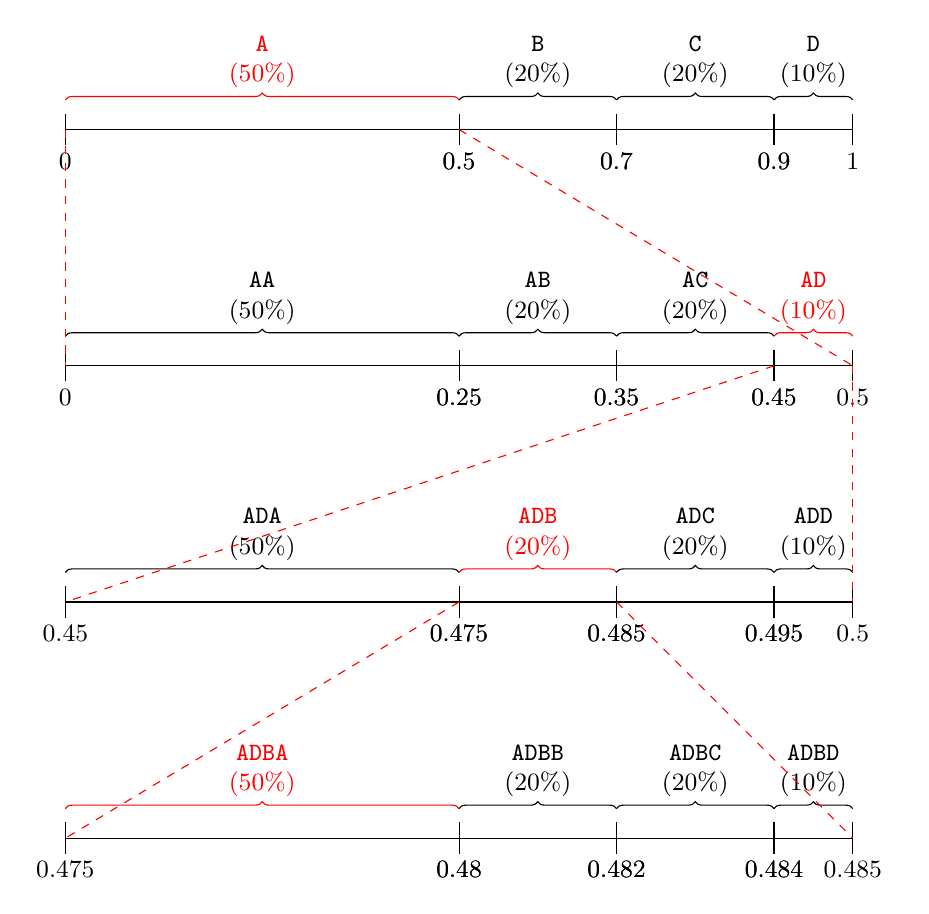
\begin{tikzpicture}
		\small\arithmeticTikz{4}{{0.5,0.2,0.2,0.1}}{{0,0.5,0.7,0.9}}{{"A","B","C","D"}}{1}{0}{1}
		\arithmeticTikz{1}{{0.5,0.2,0.2,0.1}}{{0.5,0.6,0.2,0.7}{0,0.5,0.7,0.9}}{{"AA","AB","AC","AD"}}{4}{0}{.5}
		\arithmeticTikz{-2}{{0.5,0.2,0.2,0.1}}{{0.5,0.6,0.2,0.7}{0,0.5,0.7,0.9}}{{"ADA","ADB","ADC","ADD"}}{2}{.45}{.5}
		\arithmeticTikz{-5}{{0.5,0.2,0.2,0.1}}{{0.5,0.6,0.2,0.7}{0,0.5,0.7,0.9}}{{"ADBA","ADBB","ADBC","ADBD"}}{1}{.475}{.485}

		% highlight transition area (L0 to L1)
		\draw[-, red, dashed](0*10,4)--(0*10,1);
		\draw[-, red, dashed](.5*10,4)--(1*10,1);

		% highlight transition area (L1 to L2)
		\draw[-, red, dashed](.9*10,1)--(0*10,-2);
		\draw[-, red, dashed](1*10,1)--(1*10,-2);

		% highlight transition area (L2 to L3)
		\draw[-, red, dashed](.5*10,-2)--(0*10,-5);
		\draw[-, red, dashed](.7*10,-2)--(1*10,-5);
	\end{tikzpicture}
	\caption{Arithmetische Kodierung des Worts \texttt{ADBA}}
	\label{fig:arithm-kod}
\end{figure}
Der Text \enquote{\texttt{ADBA}} wird also durch das Intervall $[0.475, 0.48)$ kodiert.

\textbf{Vom Intervall zur Bitfolge}: Gespeichert wird nicht das ganze Intervall, sondern eine einzige Zahl darin, und zwar eine mit möglichst wenigen Nachkommastellen im Zweiersystem. Mit $k$ Nachkommastellen lassen sich genau die Vielfachen von $\frac{1}{2^k}$ darstellen. Mit 6 Stellen liegt kein Vielfaches von $\frac{1}{64}$ im Intervall: $\frac{30}{64}=0.46875$ ist zu klein, $\frac{31}{64}=0.484375$ zu gross. Mit 7 Stellen passt $\frac{61}{128}=0.4765625$:
\[0.4765625 = 0.0111101_2\]
Gespeichert werden also die 7 Bits \texttt{0111101} und die Textlänge 4. Eine Huffman-Kodierung für diese Häufigkeiten (A $=$ \texttt{0}, C $=$ \texttt{10}, B $=$ \texttt{110}, D $=$ \texttt{111}) braucht für \texttt{ADBA} 8 Bits.

\textbf{Dekodieren}: Um aus der Zahl $0.4765625$ und der Textlänge 4 den Text zurückzugewinnen, sucht man in \cref{fig:arithm-kod} Zeile für Zeile das Teilintervall, in dem die Zahl liegt. Sie liegt in $[0, 0.5)$, also ist der erste Buchstabe A. Danach liegt sie in $[0.45, 0.5)$ (\texttt{AD}), in $[0.475, 0.485)$ (\texttt{ADB}) und schliesslich in $[0.475, 0.48)$ (\texttt{ADBA}). Nach vier Buchstaben hört man auf. Ohne die Textlänge wüsste man nicht, wann der Text zu Ende ist, denn die Zahl liegt z.\,B. auch im Intervall von \texttt{ADBAA}. Ist statt einer Zahl ein Intervall gegeben, dekodiert man so lange, bis das Intervall des Texts mit dem gegebenen Intervall übereinstimmt.
\end{myexample}

Die arithmetische Kodierung kommt oft mit weniger Bits aus als Huffman, braucht dafür aber mehr Rechenaufwand. Beim Komprimieren und beim Dekomprimieren muss für jedes Zeichen ein neues Teilintervall mit immer mehr Nachkommastellen berechnet werden, während Huffman pro Zeichen nur ein Codewort nachschlägt. Man wägt also zwischen Speicherplatz und Rechenaufwand ab.

\begin{myexercise}
	Bestimmen Sie für die Wörter \texttt{BAD}, \texttt{BADAC} und \texttt{ACAB} jeweils das Intervall der arithmetischen Kodierung (wie in \cref{ex:arithm-adba}) basierend auf folgenden Häufigkeiten:
	\begin{table}[H]
		\centering
		\begin{tabular}{ccccc}
			Buchstabe  & A    & B    & C      & D      \\\midrule
			Häufigkeit & 50\% & 25\% & 12.5\% & 12.5\%
		\end{tabular}
	\end{table}
	\begin{myanswer}
		Die einzelnen Buchstaben erhalten die Intervalle A $[0, 0.5)$, B $[0.5, 0.75)$, C $[0.75, 0.875)$ und D $[0.875, 1)$. Darin werden die Teilintervalle Schritt für Schritt bestimmt:
		\begin{center}
			\begin{tabular}{ll}
				Text & Intervall \\\midrule
				\texttt{B} & $[0.5, 0.75)$ \\
				\texttt{BA} & $[0.5, 0.625)$ \\
				\texttt{BAD} & $[0.609375, 0.625)$ \\
				\texttt{BADA} & $[0.609375, 0.6171875)$ \\
				\texttt{BADAC} & $[0.615234375, 0.6162109375)$ \\
				\midrule
				\texttt{A} & $[0, 0.5)$ \\
				\texttt{AC} & $[0.375, 0.4375)$ \\
				\texttt{ACA} & $[0.375, 0.40625)$ \\
				\texttt{ACAB} & $[0.390625, 0.3984375)$
			\end{tabular}
		\end{center}
	\end{myanswer}
\end{myexercise}

\begin{myexercise}
	Dekomprimieren Sie die folgenden arithmetischen Kodierungen (gegeben als Zahl mit Textlänge oder als Intervall, siehe \cref{ex:arithm-adba}), wenn die Buchstabenhäufigkeitsverteilung wie folgt aussieht: A - 40\%, B - 25\%, C - 25\%, D - 10\%.
	\begin{itemize}
		\item $0.155$, Textlänge 4
		\item $[0.104, 0.144)$
		\item $[0.2, 0.21)$
		\item $0.2595$, Textlänge 5
	\end{itemize}
	\begin{myanswer}
		\begin{itemize}
			\item AADC, Intervall: [0.1544, 0.1584)
			\item AAC
			\item ABBA
			\item ABDDB, Intervall: [0.2594, 0.25965)
		\end{itemize}
	\end{myanswer}
\end{myexercise}

\begin{mychallenge}
	Lösen Sie die Challenge-Aufgaben auf Moodle zur Kompression!
\end{mychallenge}